%%%%%%%%%%%%%%%%%%%%%%%%%%%%%%%%%%%%%%%%%
% Cleese Assignment (For Students)
% LaTeX Template
% Version 2.0 (27/5/2018)
%
% This template originates from:
% http://www.LaTeXTemplates.com
%
% Author:
% Vel (vel@LaTeXTemplates.com)
%
% License:
% CC BY-NC-SA 3.0 (http://creativecommons.org/licenses/by-nc-sa/3.0/)
% 
%%%%%%%%%%%%%%%%%%%%%%%%%%%%%%%%%%%%%%%%%

%----------------------------------------------------------------------------------------
%	PACKAGES AND OTHER DOCUMENT CONFIGURATIONS
%----------------------------------------------------------------------------------------

\documentclass[11pt]{article}
\usepackage{float}

% \usepackage[printwatermark]{xwatermark}
% \newwatermark[allpages,color=gray!50,angle=45,scale=2.5,xpos=-5,ypos=-5]{Mohammad Hadi}

%%%%%%%%%%%%%%%%%%%%%%%%%%%%%%%%%%%%%%%%%
% Cleese Assignment
% Structure Specification File
% Version 1.0 (27/5/2018)
%
% This template originates from:
% http://www.LaTeXTemplates.com
%
% Author:
% Vel (vel@LaTeXTemplates.com)
%
% License:
% CC BY-NC-SA 3.0 (http://creativecommons.org/licenses/by-nc-sa/3.0/)
% 
%%%%%%%%%%%%%%%%%%%%%%%%%%%%%%%%%%%%%%%%%

%----------------------------------------------------------------------------------------
%	PACKAGES AND OTHER DOCUMENT CONFIGURATIONS
%----------------------------------------------------------------------------------------

\usepackage{lastpage} % Required to determine the last page number for the footer

\usepackage{graphicx} % Required to insert images

\setlength\parindent{0pt} % Removes all indentation from paragraphs

\usepackage[most]{tcolorbox} % Required for boxes that split across pages

\usepackage{booktabs} % Required for better horizontal rules in tables

\usepackage{listings} % Required for insertion of code

\usepackage{etoolbox} % Required for if statements

%----------------------------------------------------------------------------------------
%	MARGINS
%----------------------------------------------------------------------------------------

\usepackage{geometry} % Required for adjusting page dimensions and margins

\geometry{
	paper=a4paper, % Change to letterpaper for US letter
	top=3cm, % Top margin
	bottom=3cm, % Bottom margin
	left=2.5cm, % Left margin
	right=2.5cm, % Right margin
	headheight=14pt, % Header height
	footskip=1.4cm, % Space from the bottom margin to the baseline of the footer
	headsep=1.2cm, % Space from the top margin to the baseline of the header
	%showframe, % Uncomment to show how the type block is set on the page
}

%----------------------------------------------------------------------------------------
%	FONT
%----------------------------------------------------------------------------------------

\usepackage[utf8]{inputenc} % Required for inputting international characters
\usepackage[T1]{fontenc} % Output font encoding for international characters

\usepackage[sfdefault,light]{roboto} % Use the Roboto font

%----------------------------------------------------------------------------------------
%	HEADERS AND FOOTERS
%----------------------------------------------------------------------------------------

\usepackage{fancyhdr} % Required for customising headers and footers

\pagestyle{fancy} % Enable custom headers and footers

\lhead{\small\assignmentClass\ifdef{\assignmentClassInstructor}{\ (\assignmentClassInstructor):}{}\ \assignmentTitle} % Left header; output the instructor in brackets if one was set
\chead{} % Centre header
\rhead{\small\ifdef{\assignmentAuthorName}{\assignmentAuthorName}{\ifdef{\assignmentDueDate}{Due\ \assignmentDueDate}{}}} % Right header; output the author name if one was set, otherwise the due date if that was set

\lfoot{} % Left footer
\cfoot{\small Page\ \thepage\ of\ \pageref{LastPage}} % Centre footer
\rfoot{} % Right footer

\renewcommand\headrulewidth{0.5pt} % Thickness of the header rule

%----------------------------------------------------------------------------------------
%	MODIFY SECTION STYLES
%----------------------------------------------------------------------------------------

\usepackage{titlesec} % Required for modifying sections

%------------------------------------------------
% Section

\titleformat
{\section} % Section type being modified
[block] % Shape type, can be: hang, block, display, runin, leftmargin, rightmargin, drop, wrap, frame
{\Large\bfseries} % Format of the whole section
{\assignmentQuestionName~\thesection} % Format of the section label
{6pt} % Space between the title and label
{} % Code before the label

\titlespacing{\section}{0pt}{0.5\baselineskip}{0.5\baselineskip} % Spacing around section titles, the order is: left, before and after

%------------------------------------------------
% Subsection

\titleformat
{\subsection} % Section type being modified
[block] % Shape type, can be: hang, block, display, runin, leftmargin, rightmargin, drop, wrap, frame
{\itshape} % Format of the whole section
{(\alph{subsection})} % Format of the section label
{4pt} % Space between the title and label
{} % Code before the label

\titlespacing{\subsection}{0pt}{0.5\baselineskip}{0.5\baselineskip} % Spacing around section titles, the order is: left, before and after

\renewcommand\thesubsection{(\alph{subsection})}

%----------------------------------------------------------------------------------------
%	CUSTOM QUESTION COMMANDS/ENVIRONMENTS
%----------------------------------------------------------------------------------------

% Environment to be used for each question in the assignment
\newenvironment{question}{
	\vspace{0.5\baselineskip} % Whitespace before the question
	\section{} % Blank section title (e.g. just Question 2)
	\lfoot{\small\itshape\assignmentQuestionName~\thesection~continued on next page\ldots} % Set the left footer to state the question continues on the next page, this is reset to nothing if it doesn't (below)
}{
	\lfoot{} % Reset the left footer to nothing if the current question does not continue on the next page
}

%------------------------------------------------

% Environment for subquestions, takes 1 argument - the name of the section
\newenvironment{subquestion}[1]{
	\subsection{#1}
}{
}

%------------------------------------------------

% Command to print a question sentence
\newcommand{\questiontext}[1]{
	\textbf{#1}
	\vspace{0.5\baselineskip} % Whitespace afterwards
}

%------------------------------------------------

% Command to print a box that breaks across pages with the question answer
\newcommand{\answer}[1]{
	\begin{tcolorbox}[breakable, enhanced]
		#1
	\end{tcolorbox}
}

%------------------------------------------------

% Command to print a box that breaks across pages with the space for a student to answer
\newcommand{\answerbox}[1]{
	\begin{tcolorbox}[breakable, enhanced]
		\vphantom{L}\vspace{\numexpr #1-1\relax\baselineskip} % \vphantom{L} to provide a typesetting strut with a height for the line, \numexpr to subtract user input by 1 to make it 0-based as this command is
	\end{tcolorbox}
}

%------------------------------------------------

% Command to print an assignment section title to split an assignment into major parts
\newcommand{\assignmentSection}[1]{
	{
		\centering % Centre the section title
		\vspace{2\baselineskip} % Whitespace before the entire section title
		
		\rule{0.8\textwidth}{0.5pt} % Horizontal rule
		
		\vspace{0.75\baselineskip} % Whitespace before the section title
		{\LARGE \MakeUppercase{#1}} % Section title, forced to be uppercase
		
		\rule{0.8\textwidth}{0.5pt} % Horizontal rule
		
		\vspace{\baselineskip} % Whitespace after the entire section title
	}
}

%----------------------------------------------------------------------------------------
%	TITLE PAGE
%----------------------------------------------------------------------------------------

\author{\textbf{\assignmentAuthorName}} % Set the default title page author field
\date{} % Don't use the default title page date field

\title{
	\thispagestyle{empty} % Suppress headers and footers
	\vspace{0.2\textheight} % Whitespace before the title
	\textbf{\assignmentClass:\ \assignmentTitle}\\[-4pt]
	\ifdef{\assignmentDueDate}{{\small Due\ on\ \assignmentDueDate}\\}{} % If a due date is supplied, output it
	\ifdef{\assignmentClassInstructor}{{\large \textit{\assignmentClassInstructor}}}{} % If an instructor is supplied, output it
	\vspace{0.32\textheight} % Whitespace before the author name
}
 % Include the file specifying the document structure and custom commands

%----------------------------------------------------------------------------------------
%	ASSIGNMENT INFORMATION
%----------------------------------------------------------------------------------------

% Required
\newcommand{\assignmentQuestionName}{Experiment} % The word to be used as a prefix to question numbers; example alternatives: Problem, Exercise
\newcommand{\assignmentClass}{Electrical Circuits Lab (Taught by Mohammad Hadi)\\Manual 5 (Due on DDD.,\ mmm.\ dd,\ yyyy)} % Course (Lecturer)\\Assignment (Due date)
\newcommand{\assignmentTitle}{} % Assignment title or name
\newcommand{\assignmentAuthorName}{Sina Hashemi \& M.Mahdi Shokrzade\\402102668 - 402101985} % Student name\\Student number
%----------------------------------------------------------------------------------------

\begin{document}
\textbf{Network theorems can facilitate circuit analysis and design. In this experiment, you practically verify various network theorems including superposition, Thevenin-Norton equivalency, and maximum power transfer.
}
%----------------------------------------------------------------------------------------
%	TITLE PAGE
%----------------------------------------------------------------------------------------

\newcommand{\PicScale}{0.2}

\assignmentSection{Mandatory Experiments}

%----------------------------------------------------------------------------------------
%	QUESTION 1
%----------------------------------------------------------------------------------------

\begin{question}

    \questiontext{Build the circuit shown in Fig. \ref{fig:cir1} on a breadboard.}

    \begin{figure}[H]
        \centering
        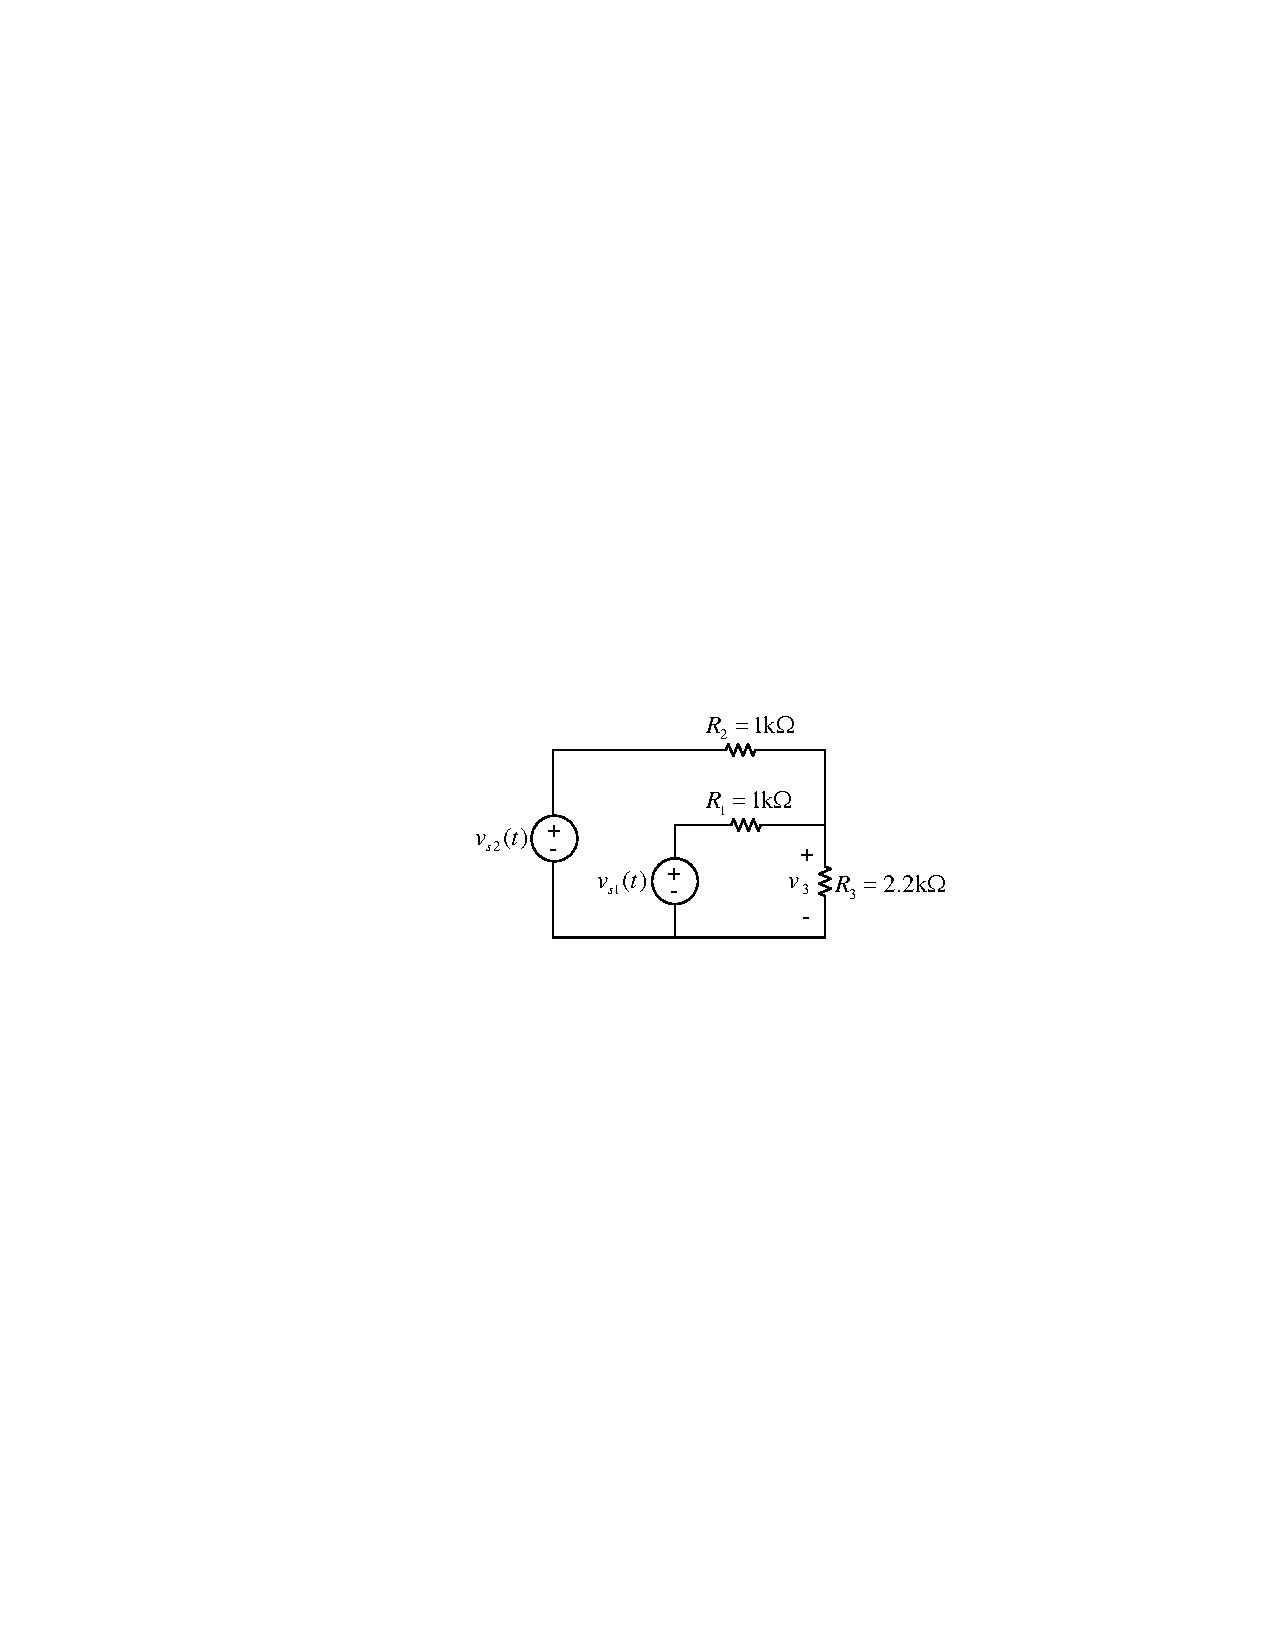
\includegraphics[scale=1.2,angle=0]{Fig/cir1.pdf}
        \caption{A circuit with two voltage sources.} \label{fig:cir1}
    \end{figure}

    %--------------------------------------------
    \begin{subquestion}{Connect $v_{s1}(t)$ and $v_{s2}(t)$ to a $5$V and $10$V DC voltage source, respectively.}
        \answer{
            \begin{figure}[H]
                \centering
                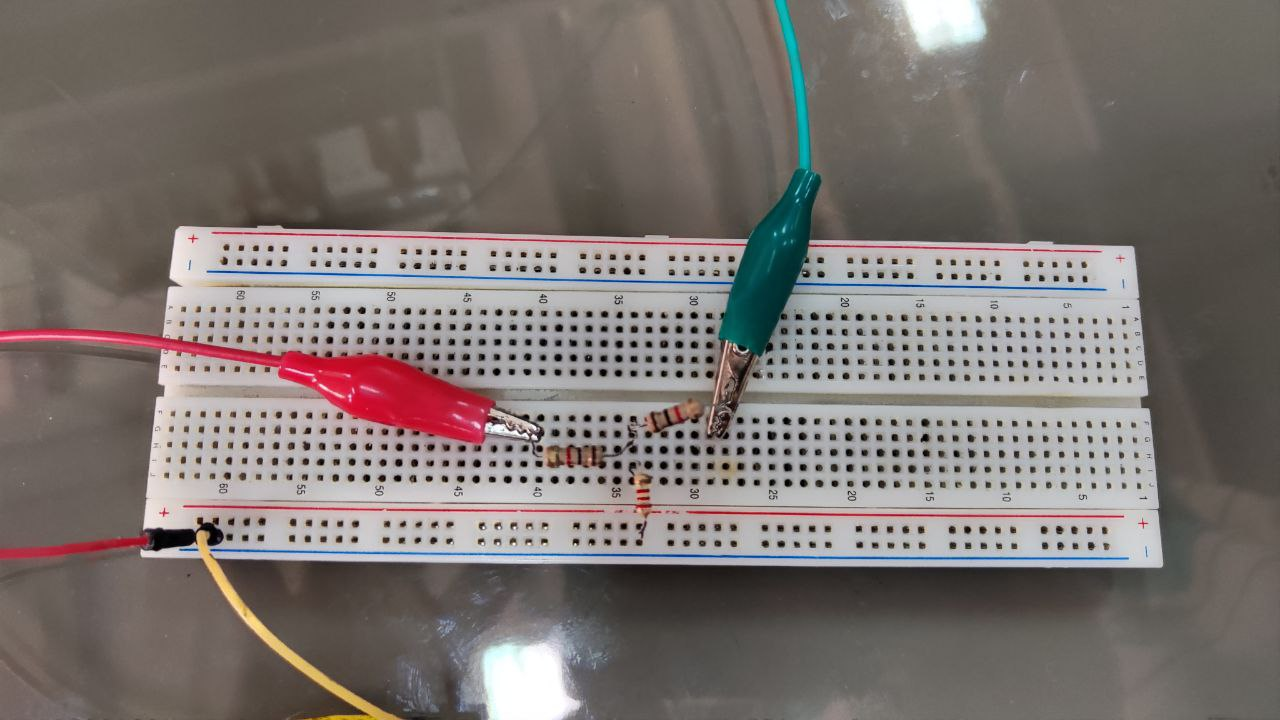
\includegraphics[scale=\PicScale,angle=0]{Fig/1.jpeg}
                \caption{The circuit.}
            \end{figure}
            \begin{figure}[H]
                \centering
                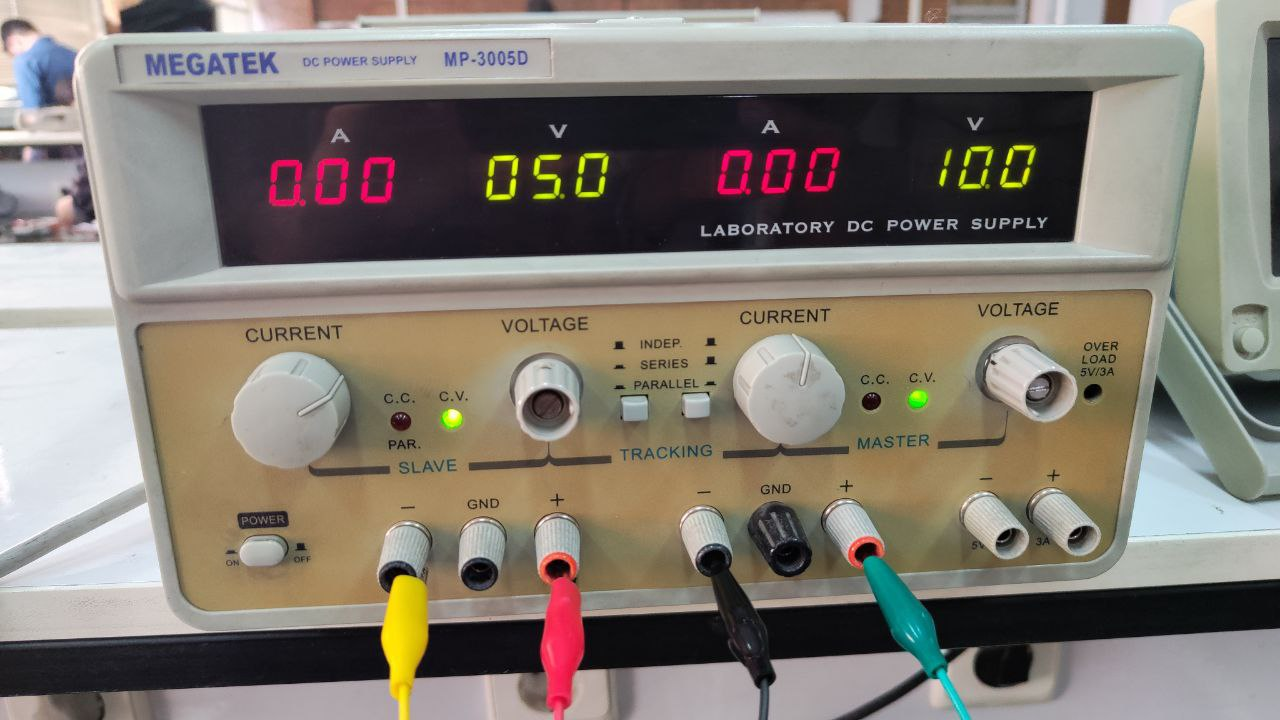
\includegraphics[scale=\PicScale,angle=0]{Fig/2.jpeg}
                \caption{The DC power supply.}
            \end{figure}
        }
    \end{subquestion}

    %--------------------------------------------
    \begin{subquestion}{Measure $v_3$ using a multimeter when $v_{s1}(t)$ is on and $v_{s2}(t)$ is off. Make sure that $v_{s2}(t)$ acts like short circuit when it is off.}
        \answer{
            \begin{figure}[H]
                \centering
                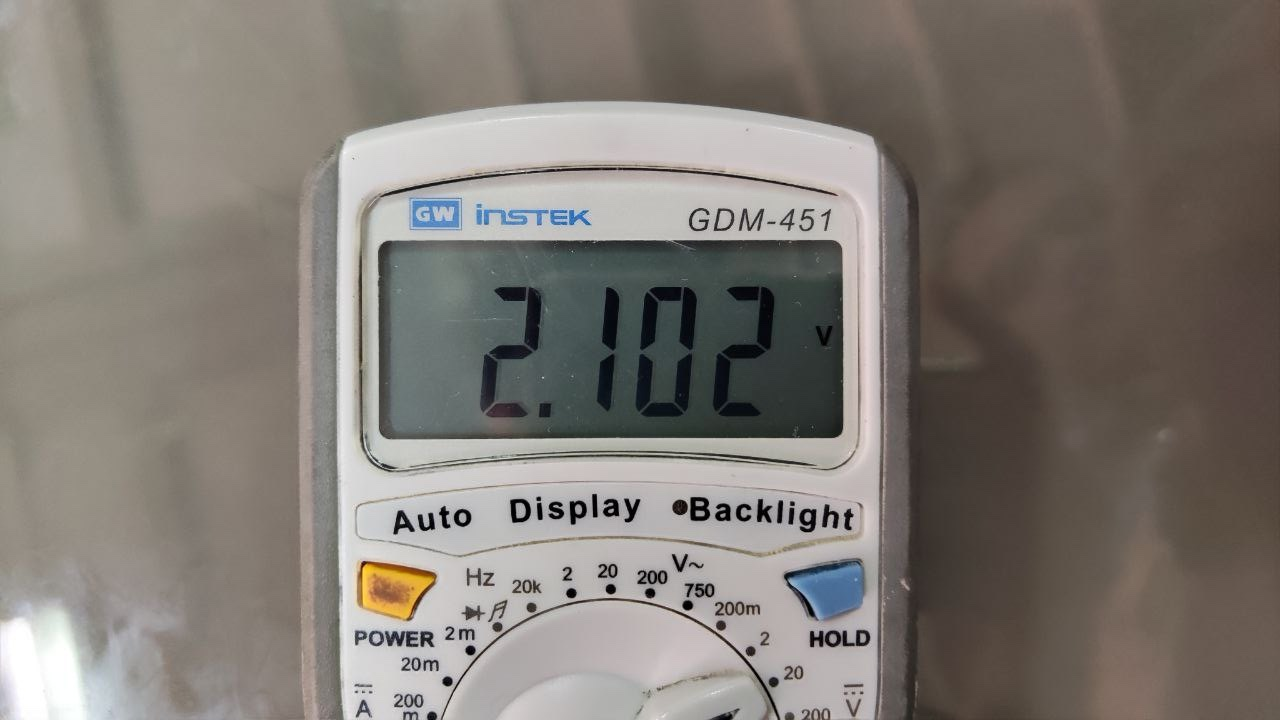
\includegraphics[scale=\PicScale,angle=0]{Fig/3.jpeg}
                \caption{...}
            \end{figure}
        }
    \end{subquestion}

    %--------------------------------------------
    \begin{subquestion}{Measure $v_3$ using a multimeter when $v_{s2}(t)$ is on and $v_{s1}(t)$ is off. Make sure that $v_{s1}(t)$ acts like short circuit when it is off.}
        \answer{
            \begin{figure}[H]
                \centering
                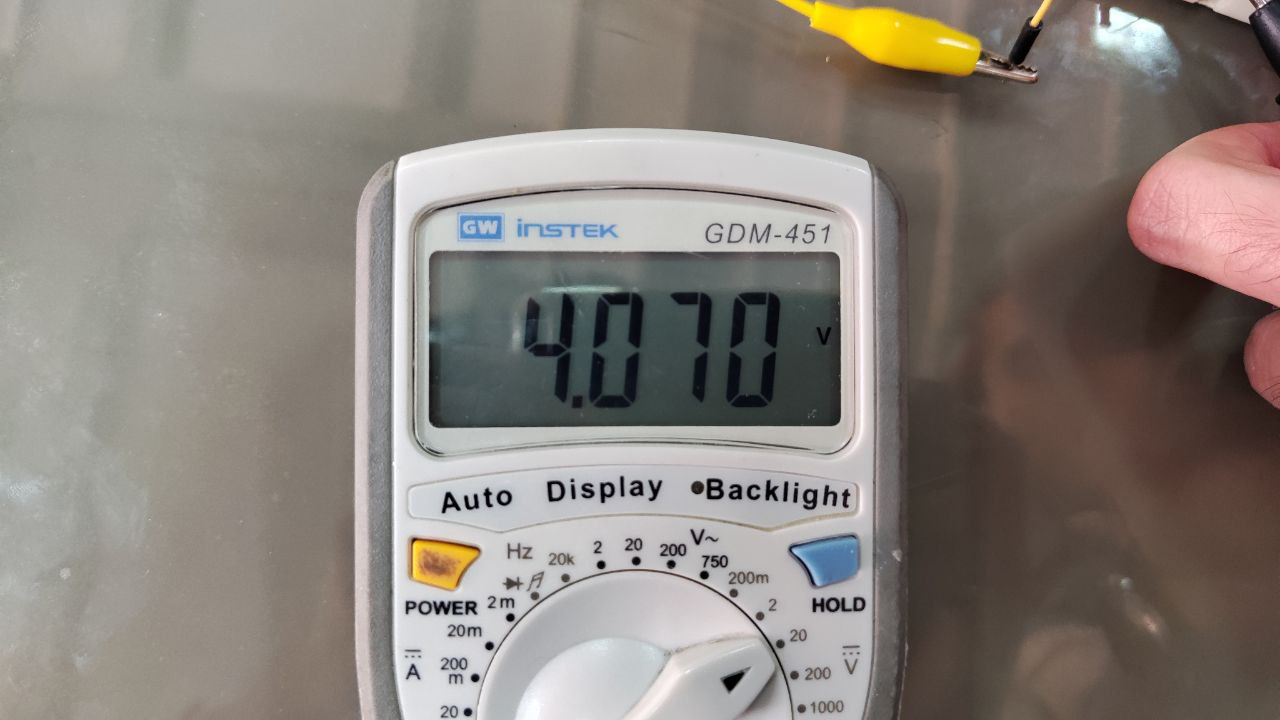
\includegraphics[scale=\PicScale,angle=0]{Fig/4.jpeg}
                \caption{...}
            \end{figure}
        }
    \end{subquestion}

    %--------------------------------------------
    \begin{subquestion}{Measure $v_3$ using a multimeter when both $v_{s1}(t)$ and $v_{s2}(t)$ are on. Verify the superposition theorem.}
        \answer{
            \begin{figure}[H]
                \centering
                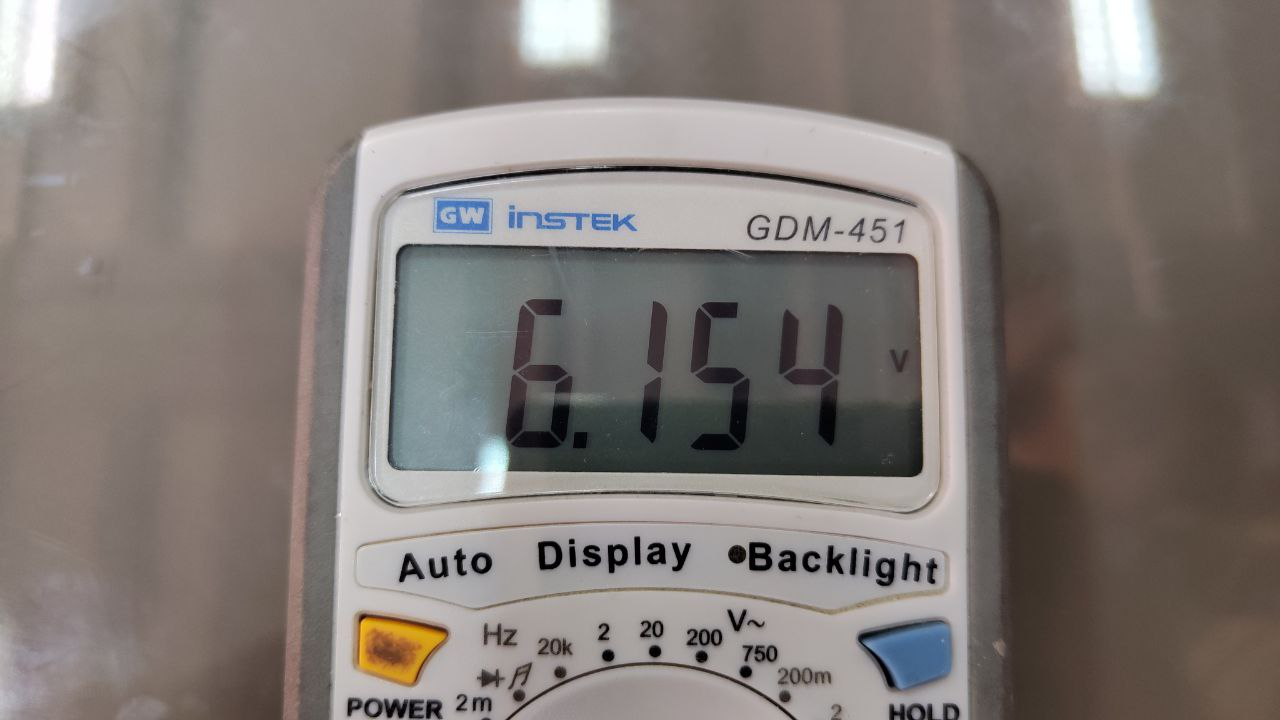
\includegraphics[scale=\PicScale,angle=0]{Fig/5.jpeg}
                \caption{...}
            \end{figure}
        }
    \end{subquestion}

    %--------------------------------------------
    \begin{subquestion}{Connect $v_{s1}(t)$ and $v_{s2}(t)$ to a $5$V DC voltage source and a $2$V $1$KHz sine voltage source, respectively. Verify the superposition theorem by suitable measurements using a multimeter. Repeat this part while seeing $v_3$ using an oscilloscope.}
        \answer{
            \begin{figure}[H]
                \centering
                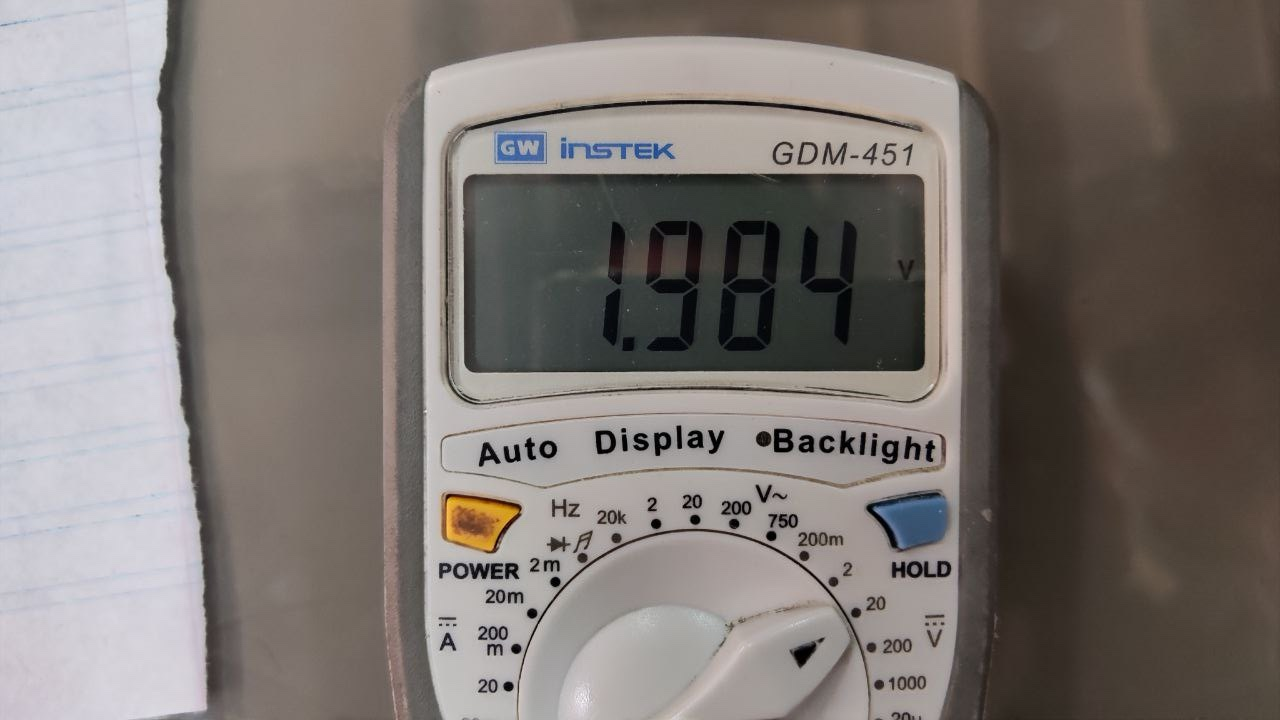
\includegraphics[scale=0.1,angle=0]{Fig/6.jpeg}
                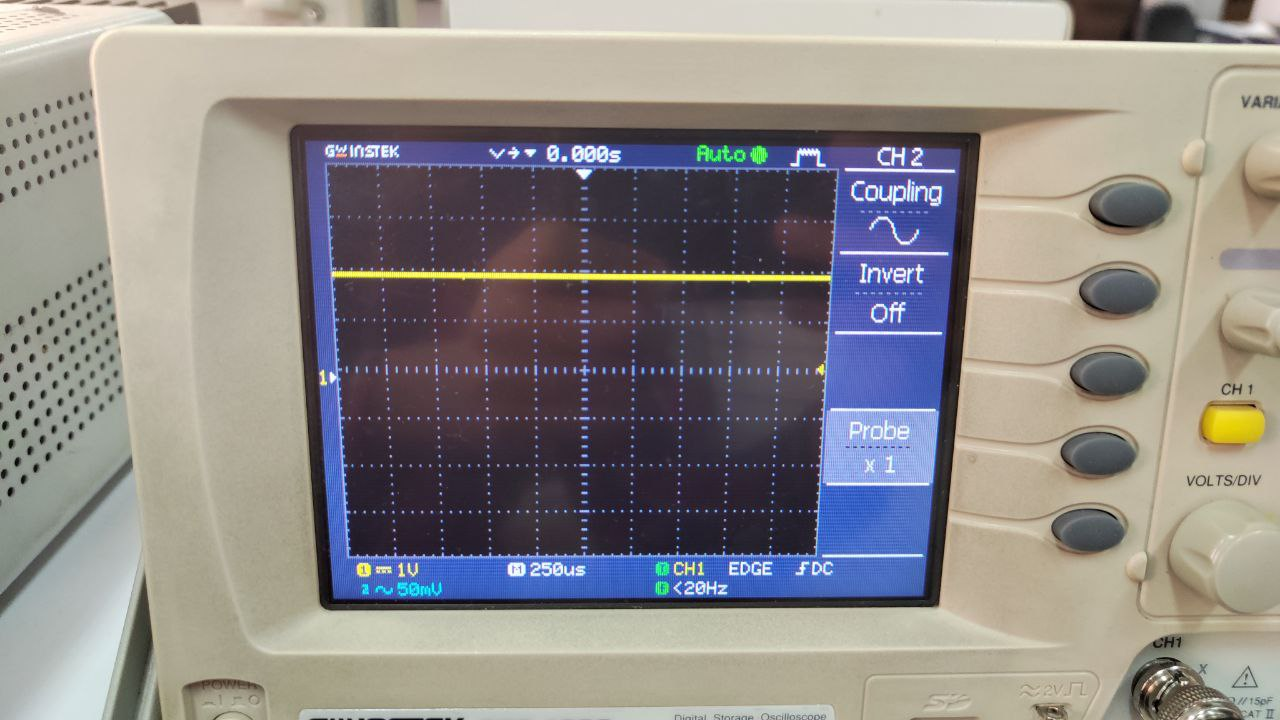
\includegraphics[scale=0.1,angle=0]{Fig/9.jpeg}
                \caption{$v_{s1}$ on and $v_{s2}(t)$ off.}
            \end{figure}
            \begin{figure}[H]
                \centering
                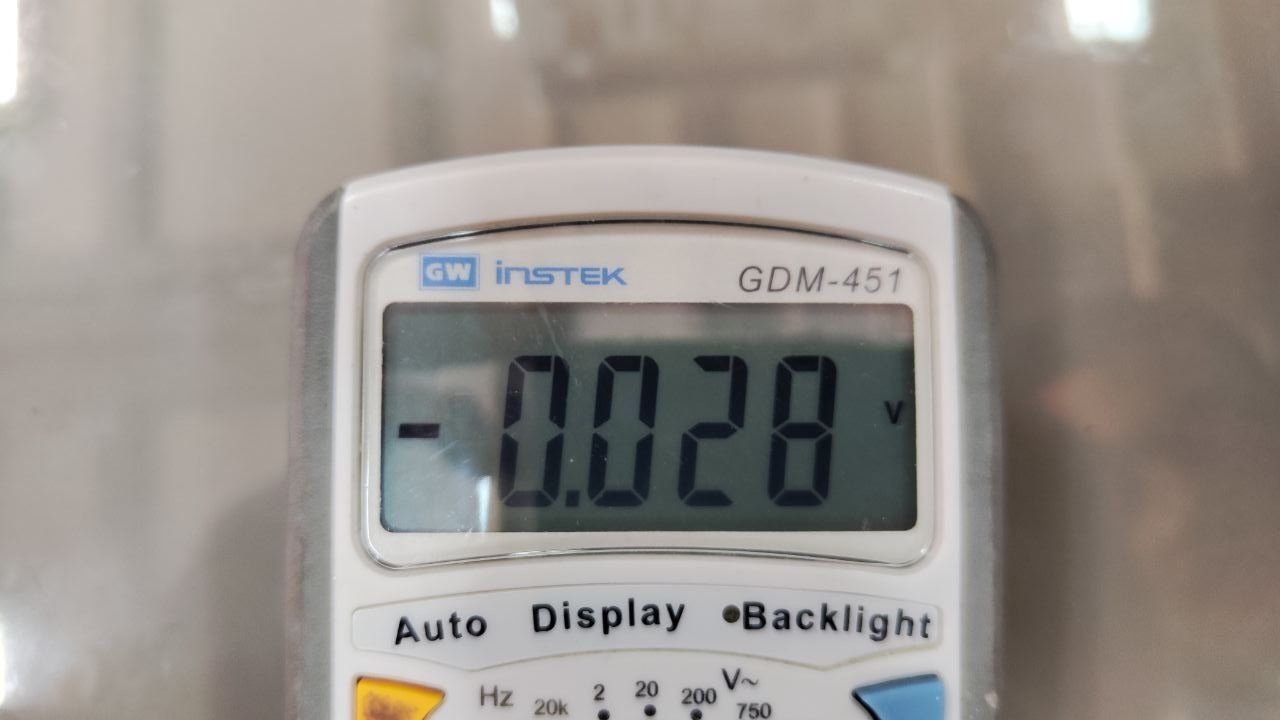
\includegraphics[scale=0.1,angle=0]{Fig/7.jpeg}
                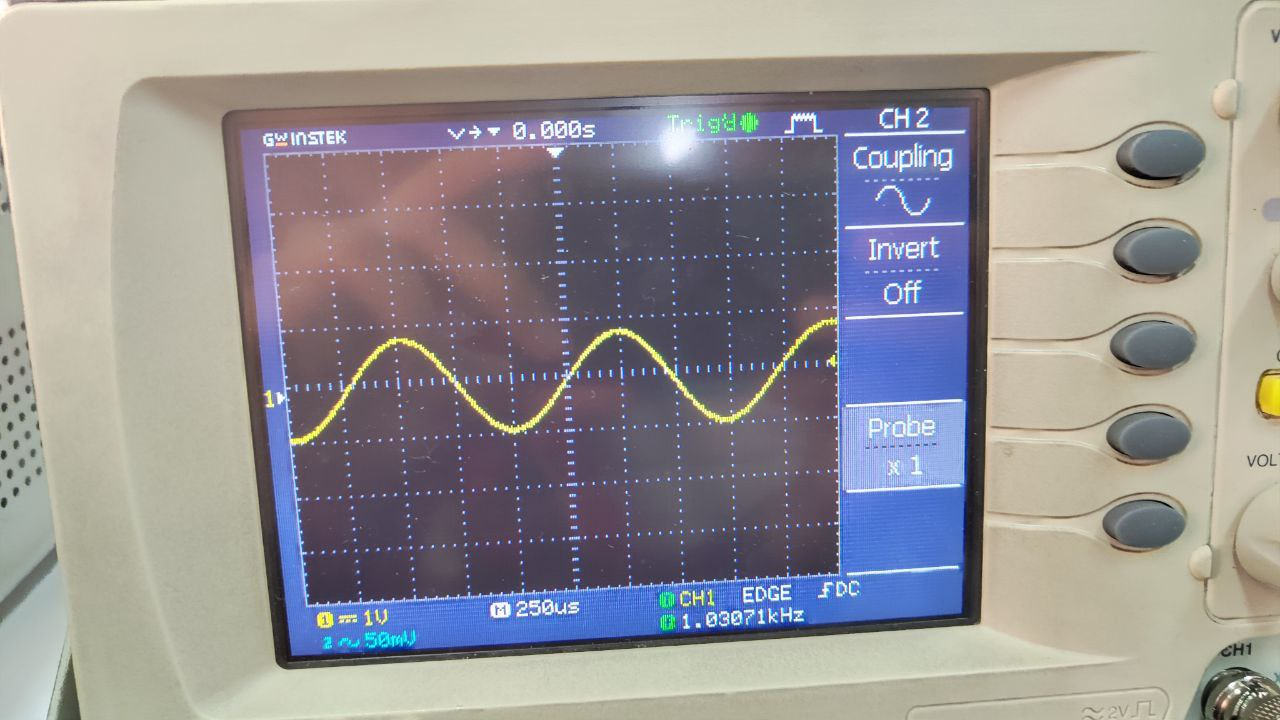
\includegraphics[scale=0.1,angle=0]{Fig/10.jpeg}
                \caption{$v_{s1}$ off and $v_{s2}(t)$ on.}
            \end{figure}
            \begin{figure}[H]
                \centering
                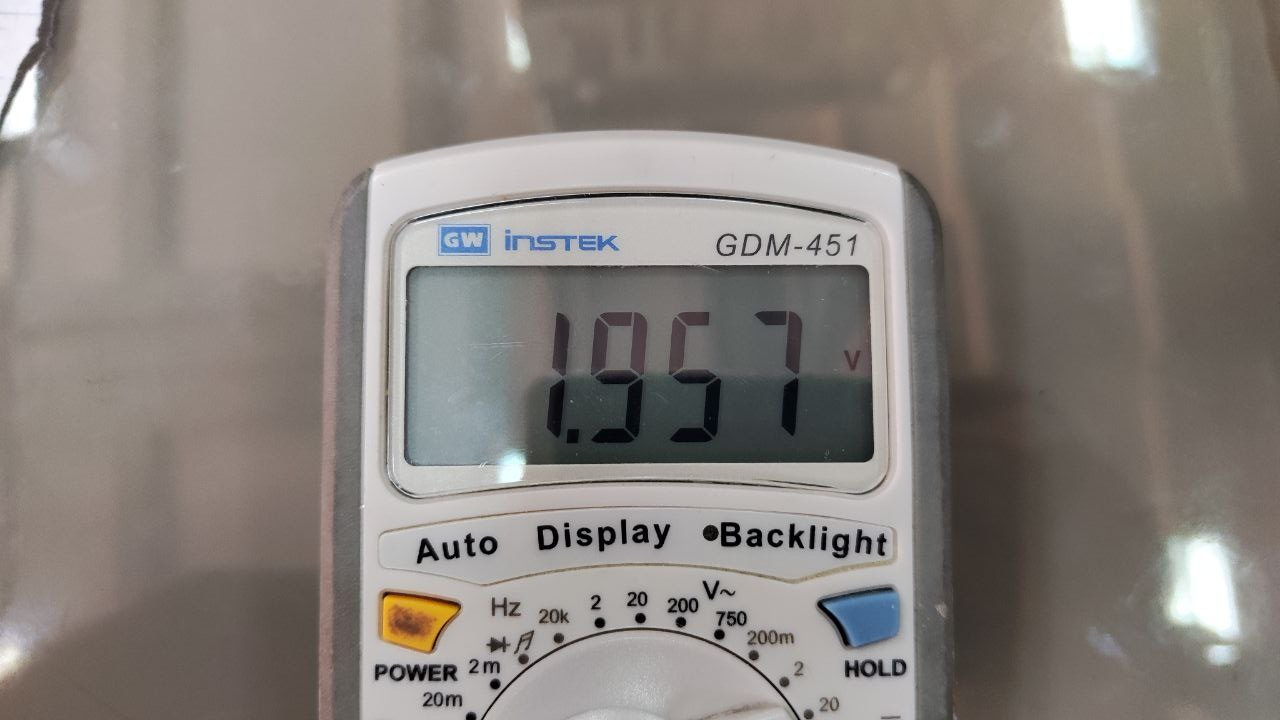
\includegraphics[scale=0.1,angle=0]{Fig/8.jpeg}
                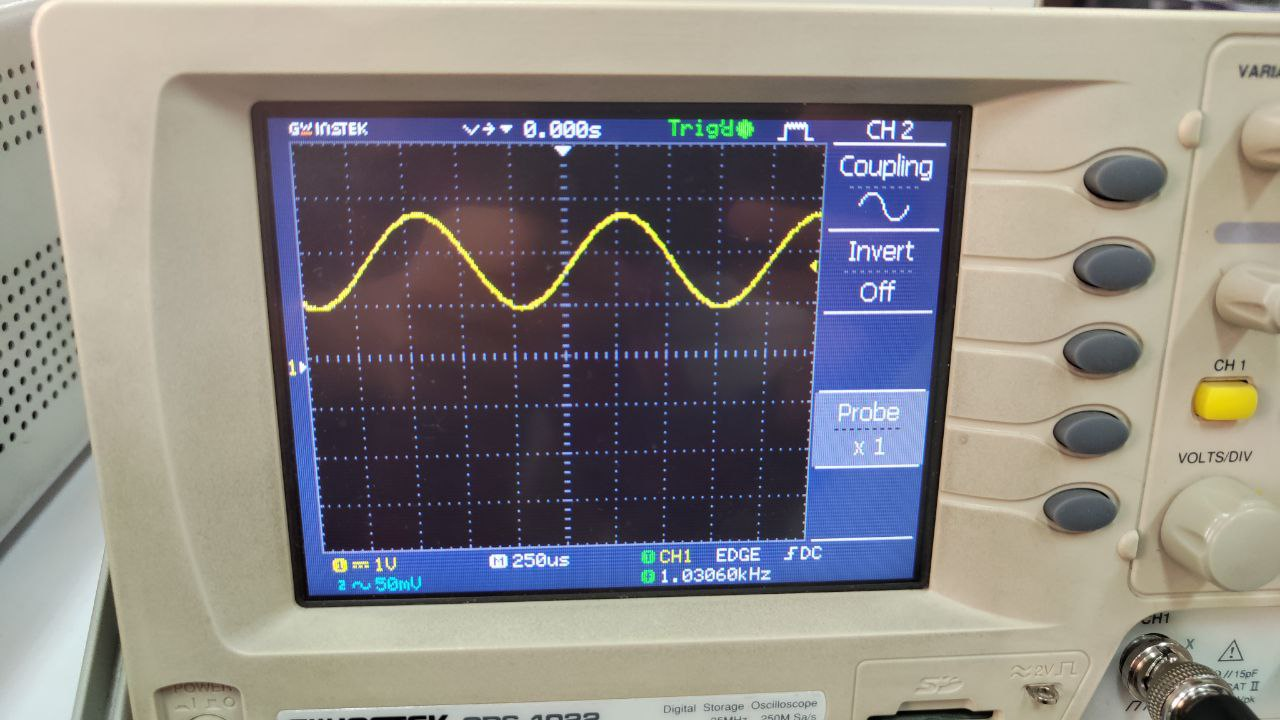
\includegraphics[scale=0.1,angle=0]{Fig/11.jpeg}
                \caption{$v_{s1}$ on and $v_{s2}(t)$ on.}
            \end{figure}
        }
    \end{subquestion}

    %--------------------------------------------
    \begin{subquestion}{Connect $v_{s1}(t)$ and $v_{s2}(t)$ to a $5$ V and $10$ V DC voltage source, respectively, and replace $R_1$ and $R_2$ with two diodes such that the positive leg of each diode connects to the positive side of the corresponding voltage source. Check if the superposition is held or not. Discuss the results.}
        \answer{
            \begin{figure}[H]
                \centering
                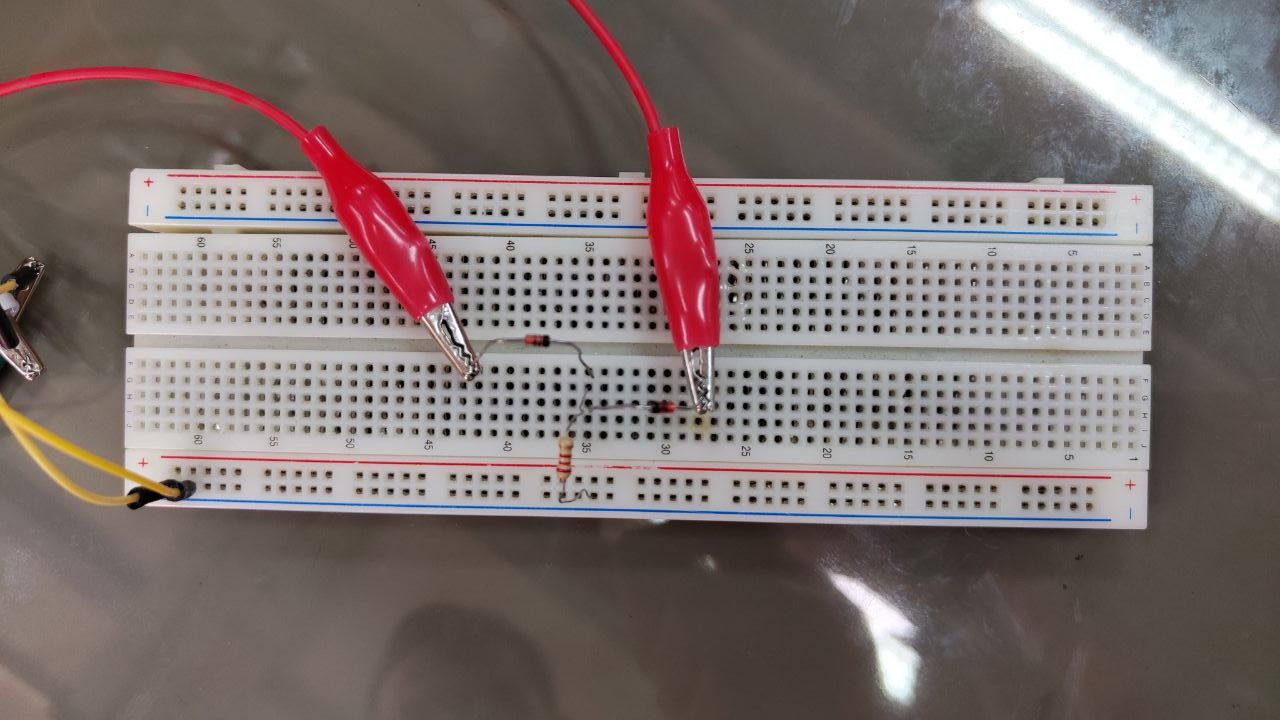
\includegraphics[scale=\PicScale,angle=0]{Fig/12.jpeg}
                \caption{The circuit.}
            \end{figure}
            \begin{figure}[H]
                \centering
                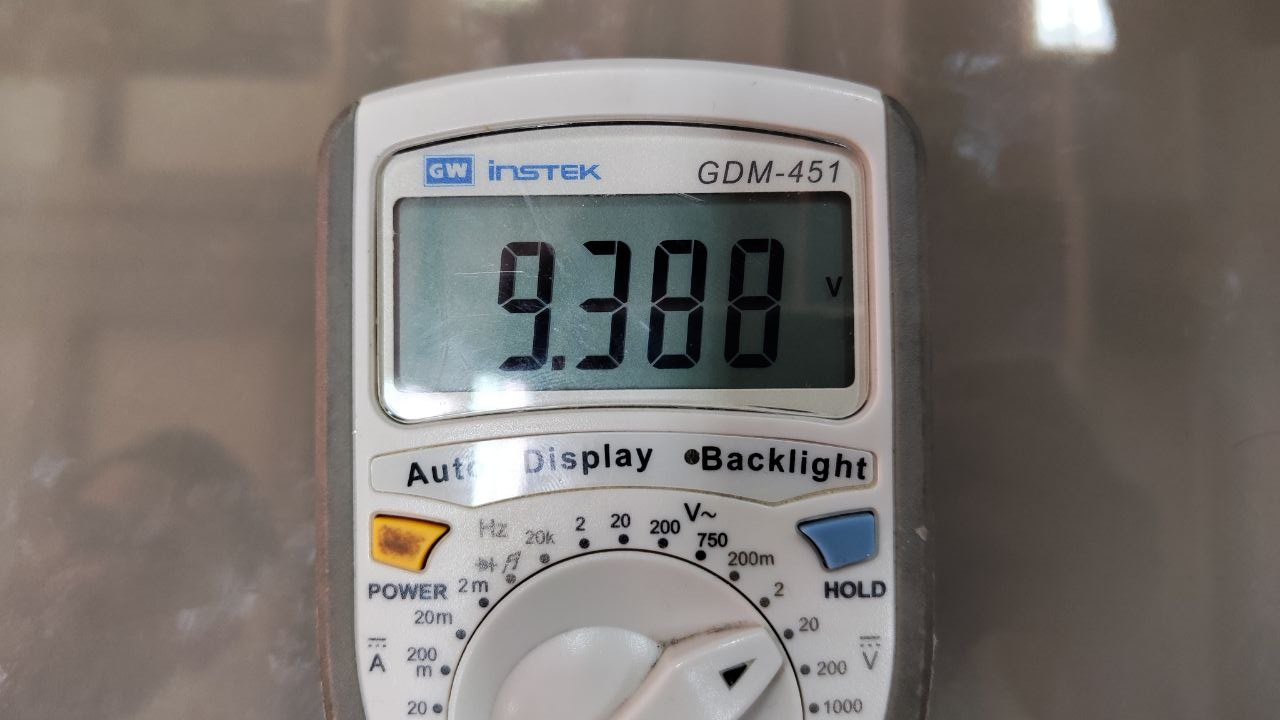
\includegraphics[scale=\PicScale,angle=0]{Fig/13.jpeg}
                \caption{$v_{s1}$ on and $v_{s2}(t)$ off.}
            \end{figure}
            \begin{figure}[H]
                \centering
                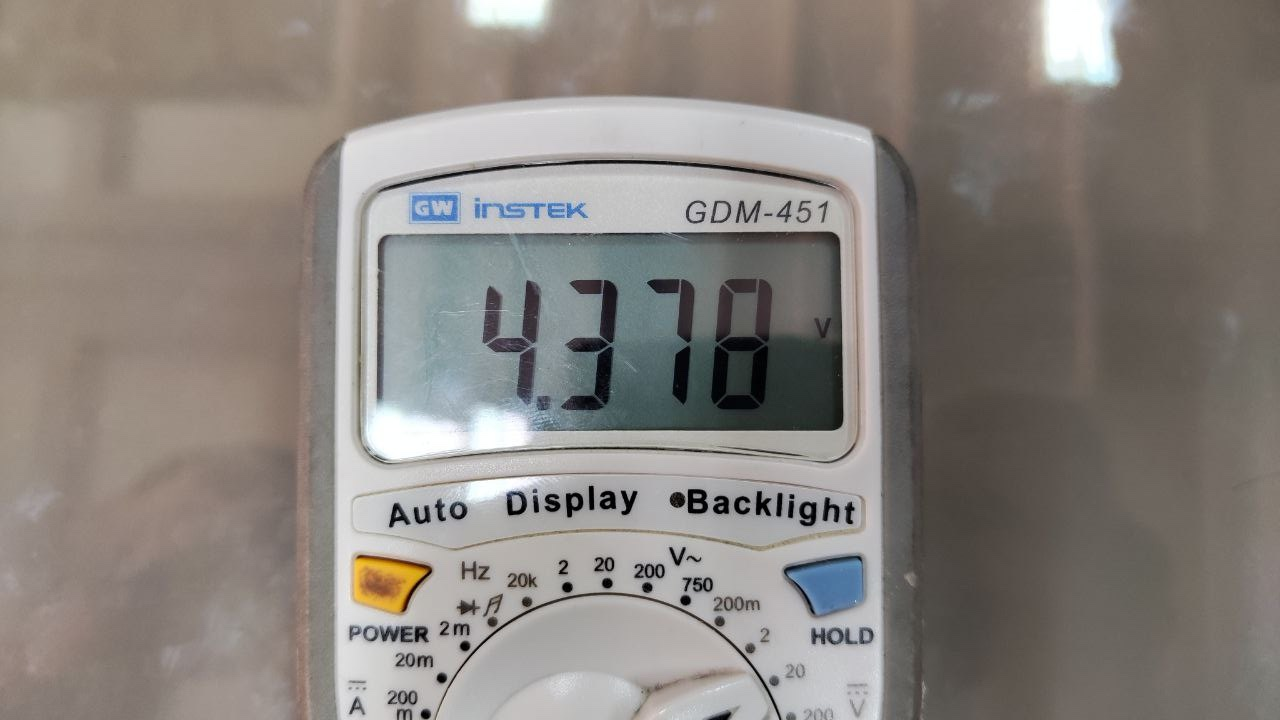
\includegraphics[scale=\PicScale,angle=0]{Fig/14.jpeg}
                \caption{$v_{s1}$ off and $v_{s2}(t)$ on.}
            \end{figure}
            \begin{figure}[H]
                \centering
                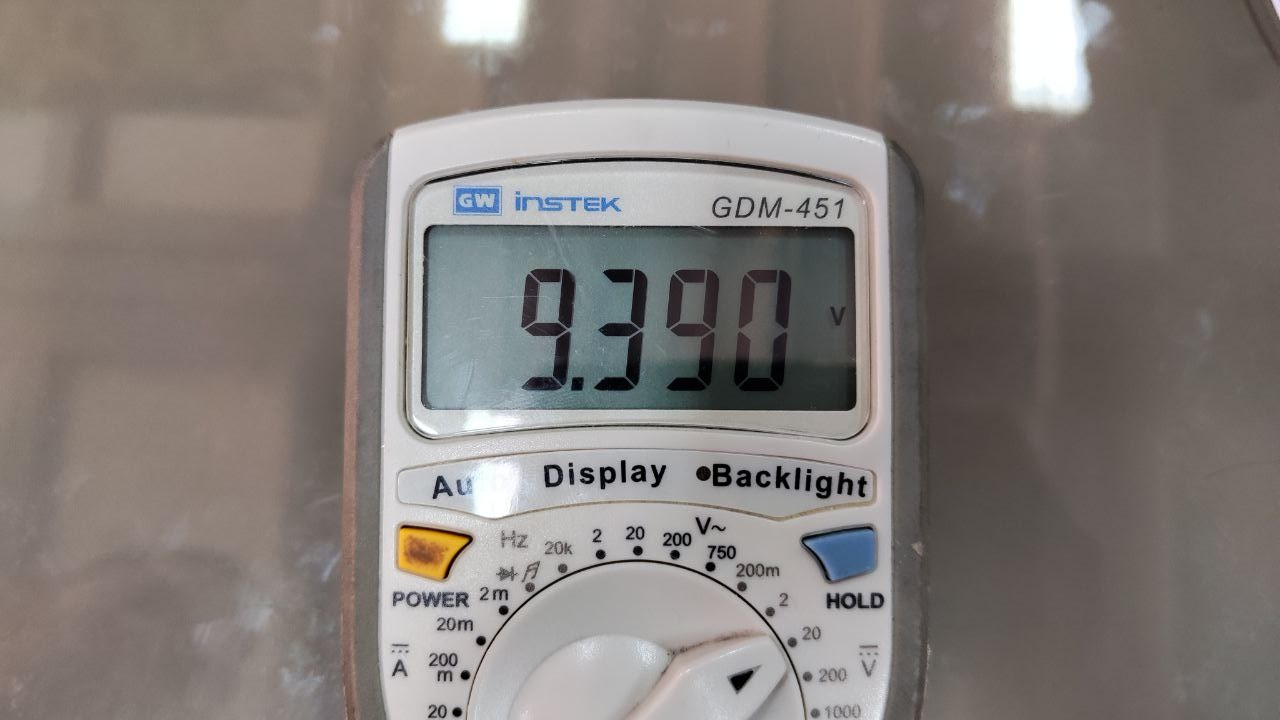
\includegraphics[scale=\PicScale,angle=0]{Fig/15.jpeg}
                \caption{$v_{s1}$ on and $v_{s2}(t)$ on.}
            \end{figure}
        }
    \end{subquestion}

\end{question}

%----------------------------------------------------------------------------------------
%	QUESTION 2
%----------------------------------------------------------------------------------------

\begin{question}

    \questiontext{Build the circuit shown in Fig. \ref{fig:cir2} on a breadboard.}

    \begin{figure}[H]
        \centering
        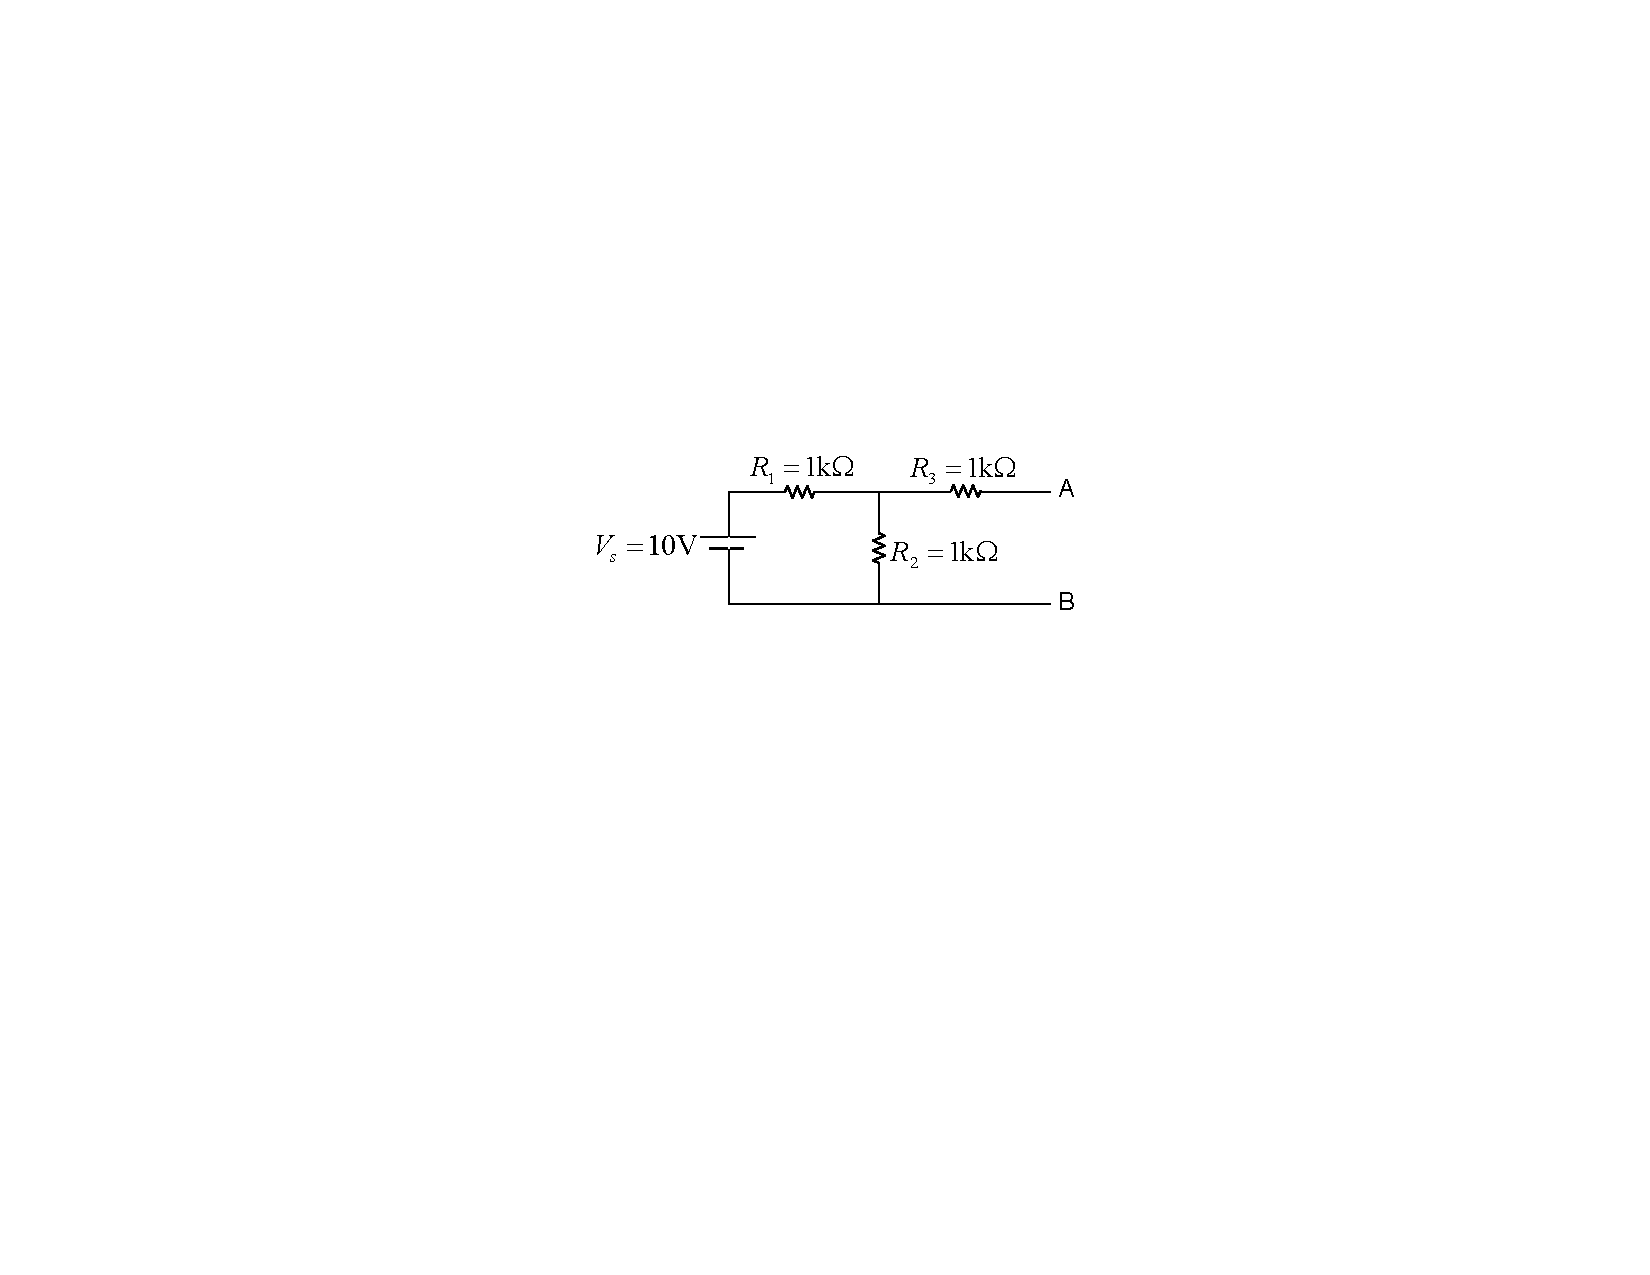
\includegraphics[scale=1.2,angle=0]{Fig/cir2.pdf}
        \caption{A linear circuit.} \label{fig:cir2}
    \end{figure}


    %--------------------------------------------
    \begin{subquestion}{Measure the open circuit voltage $V_{oc}$ of the circuit.}
        \answer{
            \begin{figure}[H]
                \centering
                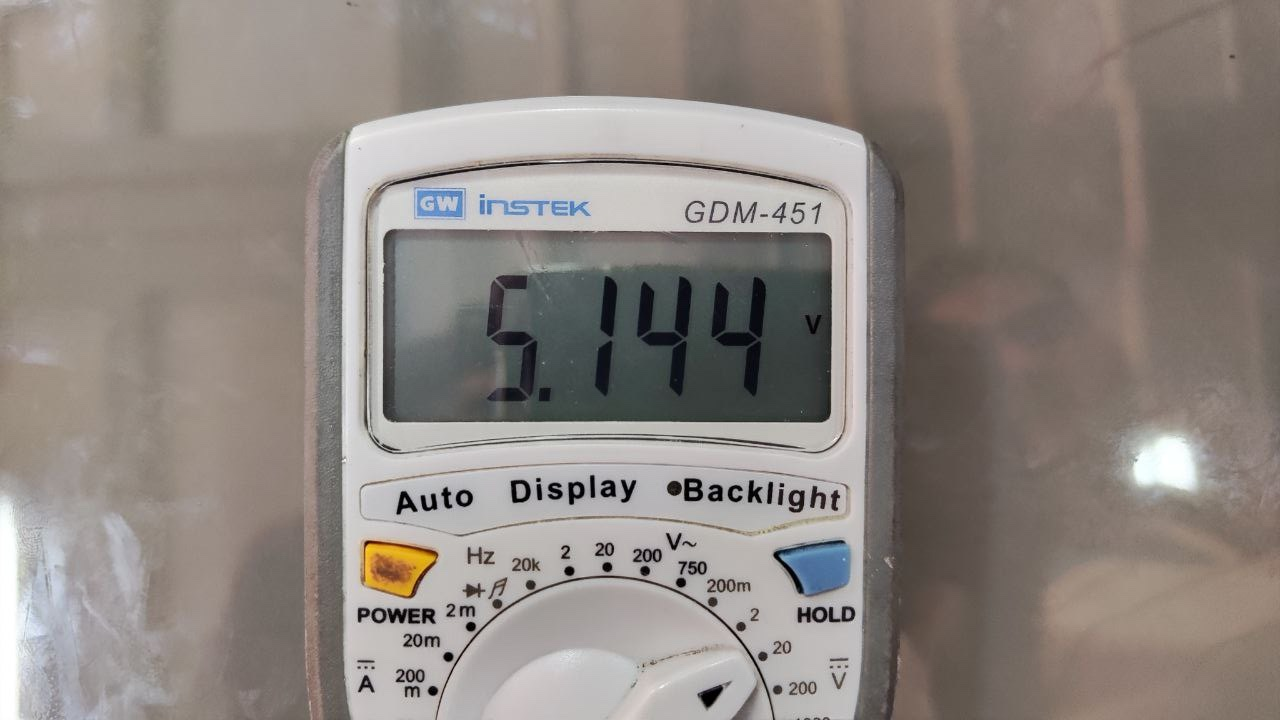
\includegraphics[scale=\PicScale,angle=0]{Fig/16.jpeg}
                \caption{...}
            \end{figure}
        }
    \end{subquestion}

    %--------------------------------------------
    \begin{subquestion}{Connect an $R_L=2.2$ k$\Omega$ resistor to the port AB and measure its voltage $V_L$.}
        \answer{
            \begin{figure}[H]
                \centering
                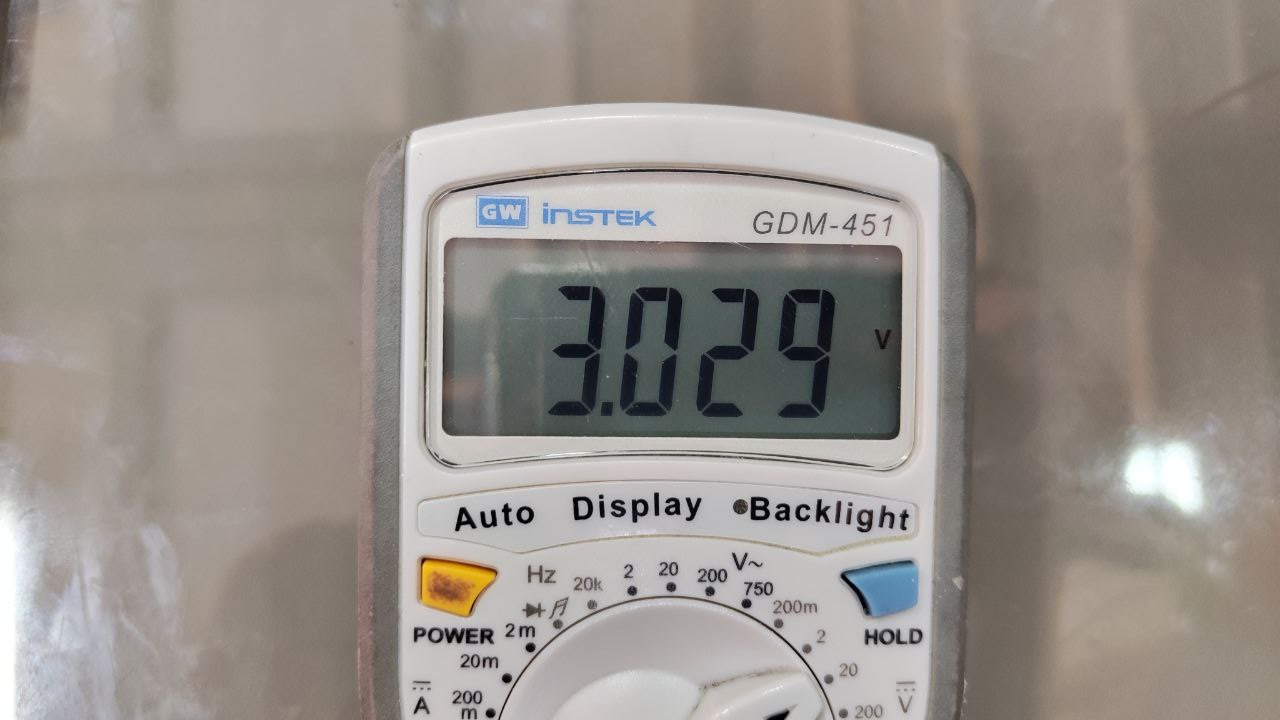
\includegraphics[scale=\PicScale,angle=0]{Fig/17.jpeg}
                \caption{...}
            \end{figure}
        }
    \end{subquestion}

    %--------------------------------------------
    \begin{subquestion}{Can you obtain the corresponding Thevenin equivalent circuit using the measured values of $V_{oc}$ and $V_L$.}
        \answer{
            \begin{figure}[H]
                \centering
                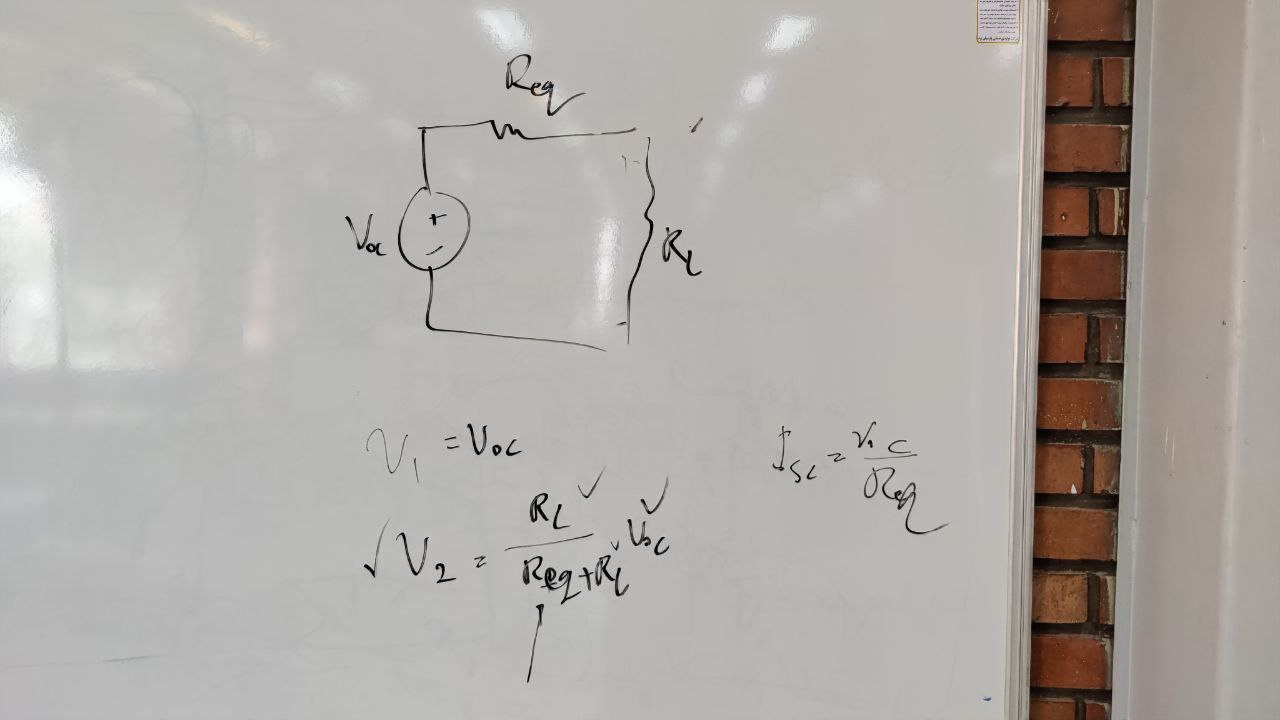
\includegraphics[scale=\PicScale,angle=0]{Fig/123456789.jpeg}
                \caption{its just for you to help you to write this part. delete it in final version.}
            \end{figure}
        }
    \end{subquestion}

    %--------------------------------------------
    \begin{subquestion}{Build the Thevenin equivalent circuit on the breadboard. Connect a same load resistor to both circuits and measure its voltage. Interpret the results.}
        \answer{
            \begin{figure}[H]
                \centering
                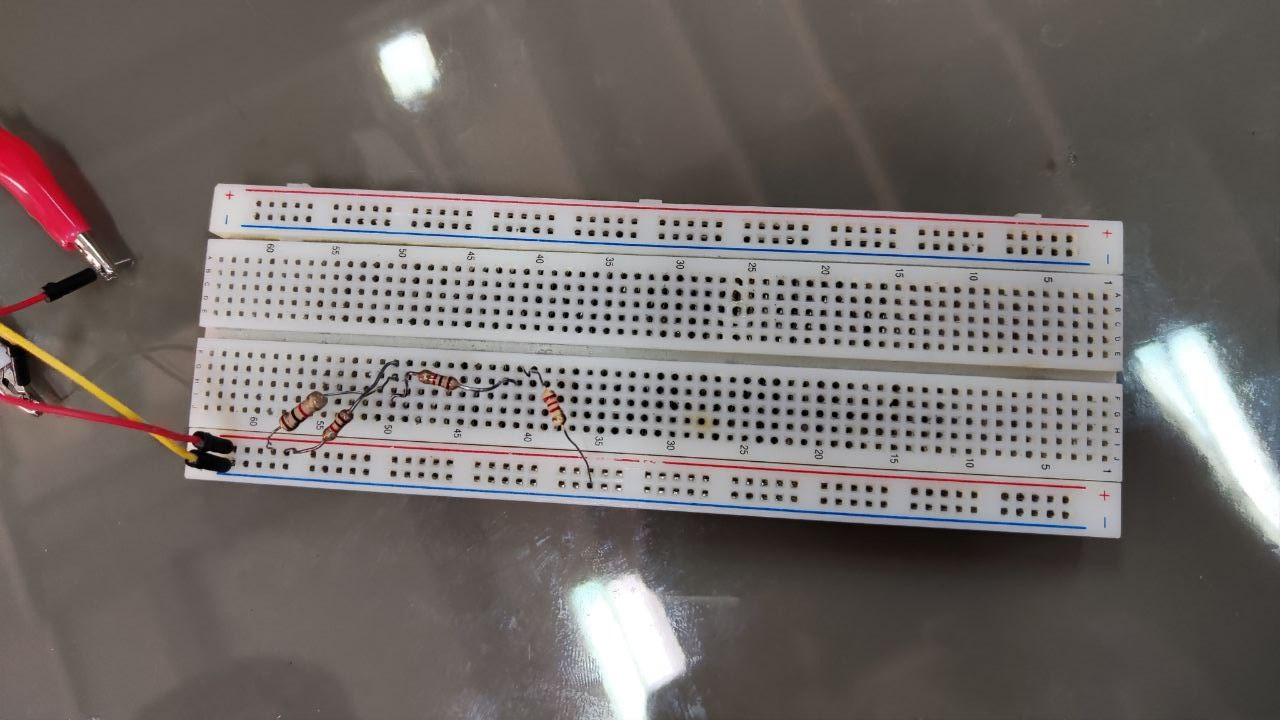
\includegraphics[scale=\PicScale,angle=0]{Fig/18.jpeg}
                \caption{The circuit.}
            \end{figure}
            \begin{figure}[H]
                \centering
                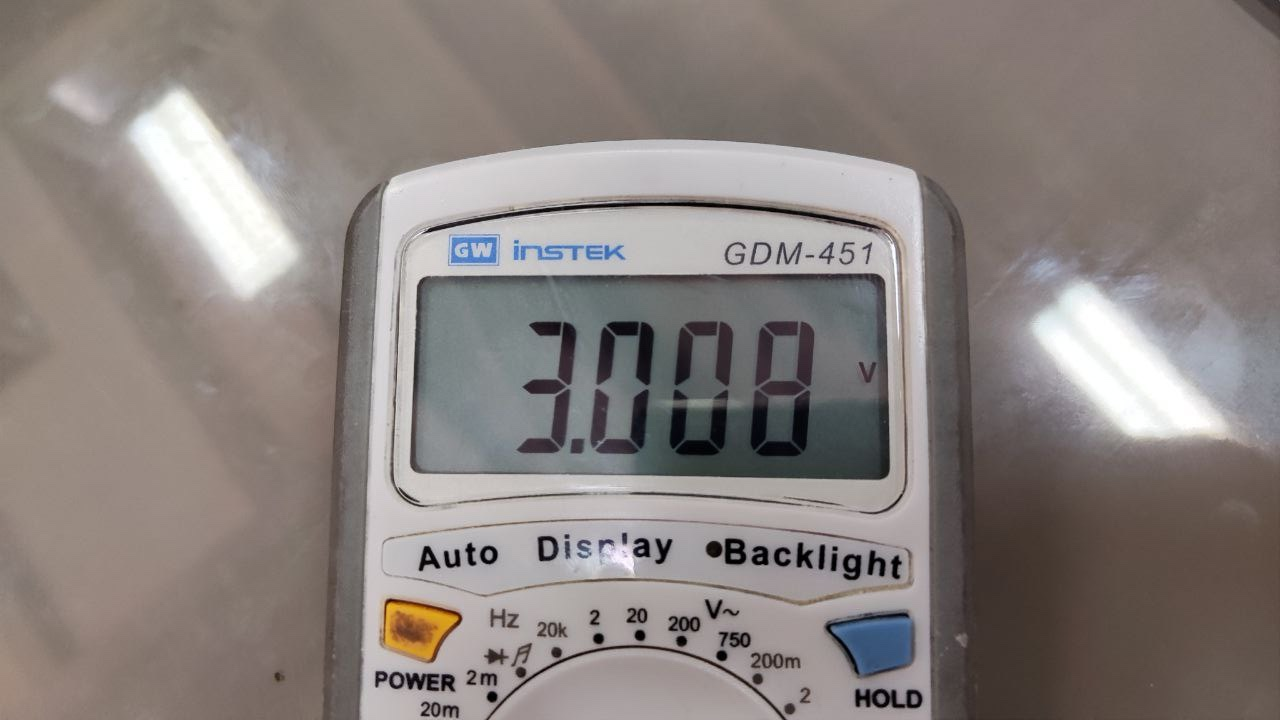
\includegraphics[scale=\PicScale,angle=0]{Fig/19.jpeg}
                \caption{Voltage of the load resistor.}
            \end{figure}
        }
    \end{subquestion}

\end{question}


%----------------------------------------------------------------------------------------
%	QUESTION 3
%----------------------------------------------------------------------------------------

\begin{question}

    \questiontext{Build the circuit shown in Fig. \ref{fig:cir3} on a breadboard.}

    \begin{figure}[H]
        \centering
        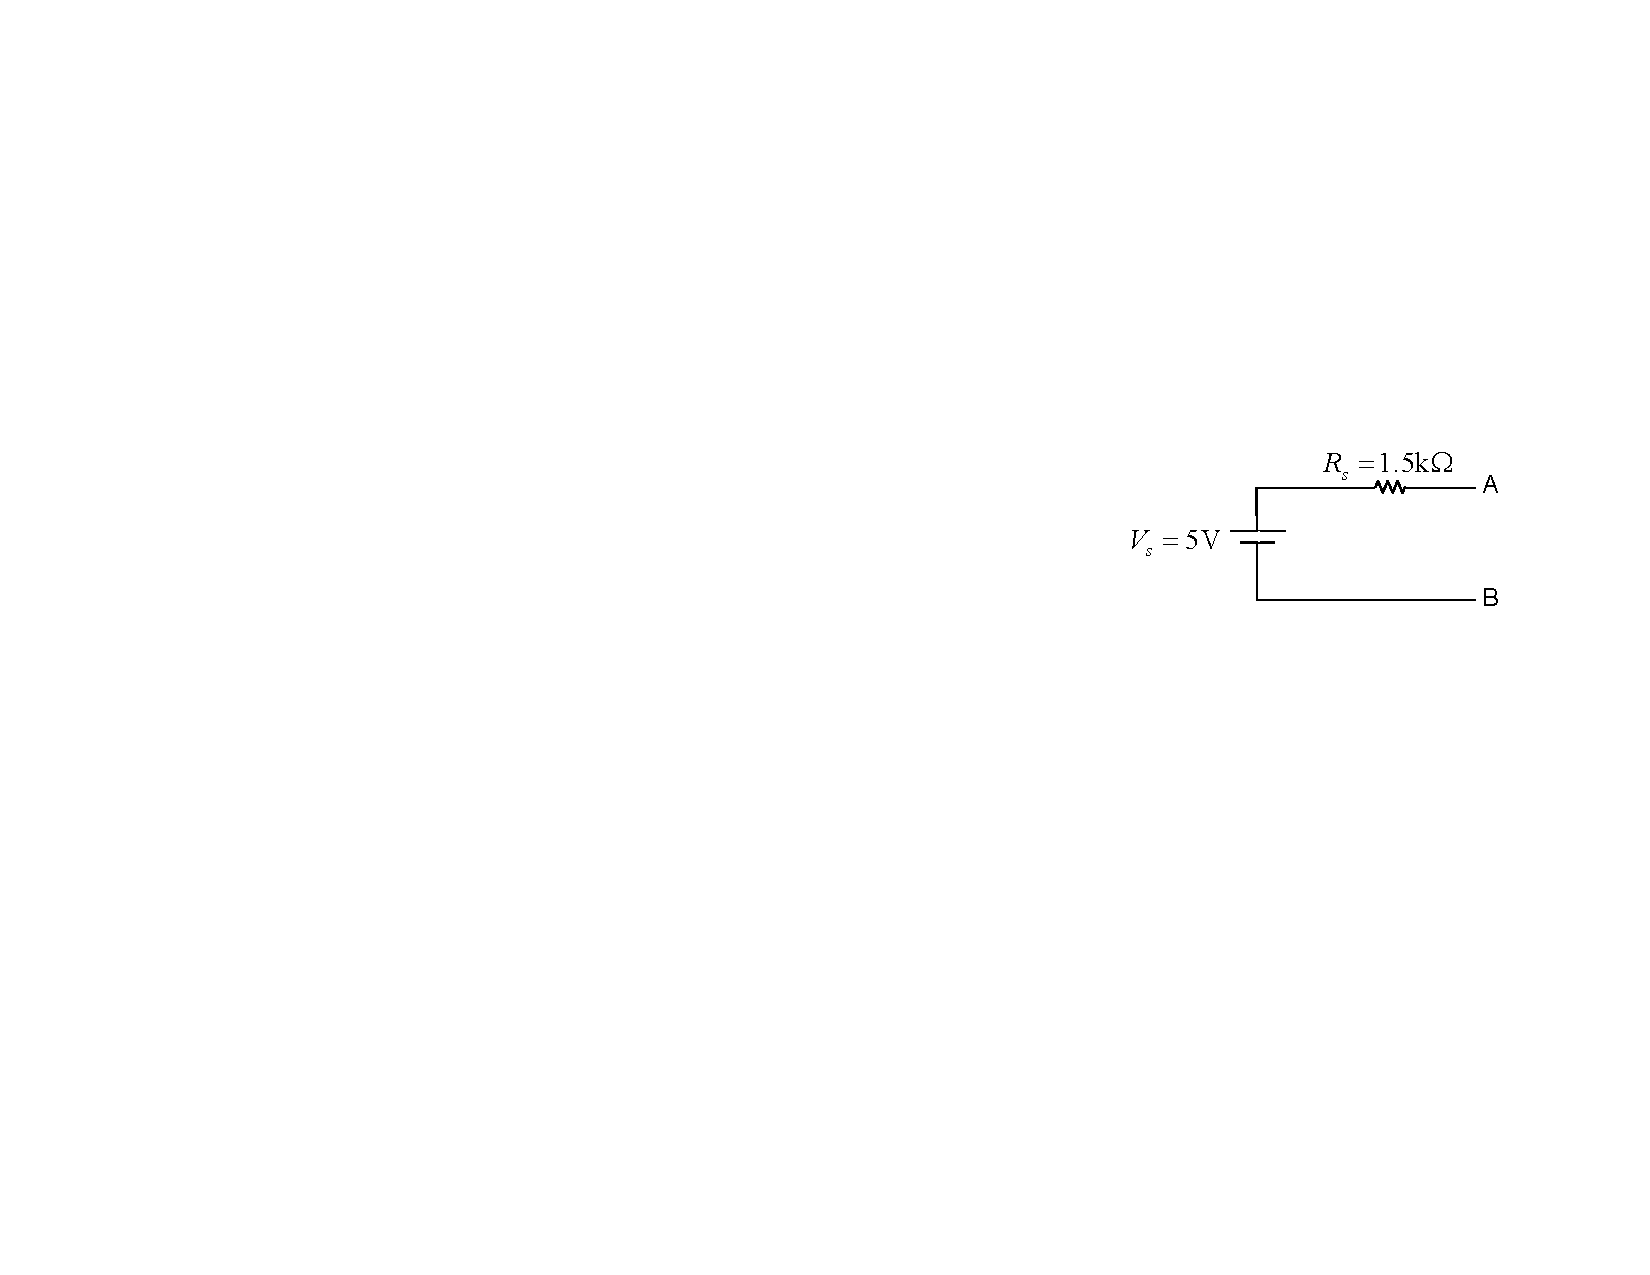
\includegraphics[scale=1.2,angle=0]{Fig/cir3.pdf}
        \caption{A simple resistive circuit.} \label{fig:cir3}
    \end{figure}


    %--------------------------------------------
    \begin{subquestion}{Calculate the load resistor $R_L$ drawing the maximum power from the source. Connect it to the port AB and measure the consumed power.}
        \answer{
            \begin{figure}[H]
                \centering
                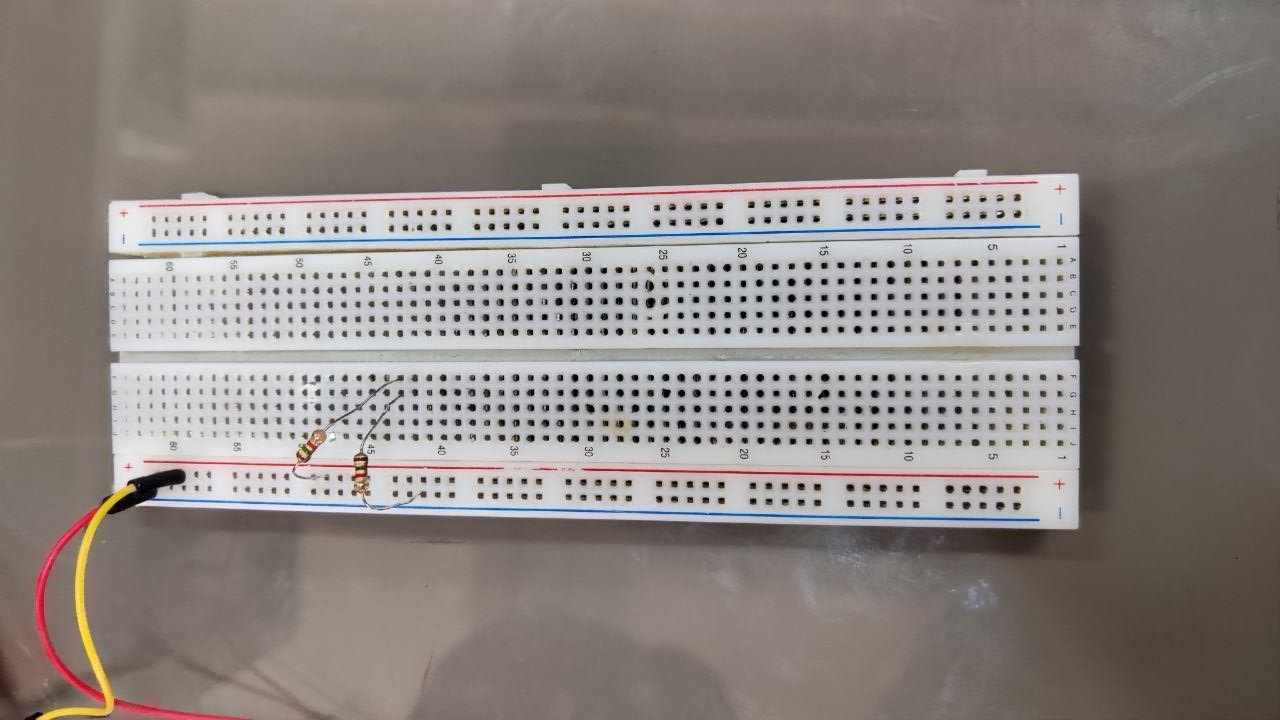
\includegraphics[scale=\PicScale,angle=0]{Fig/20.jpeg}
                \caption{The circuit.}
            \end{figure}
            \begin{figure}[H]
                \centering
                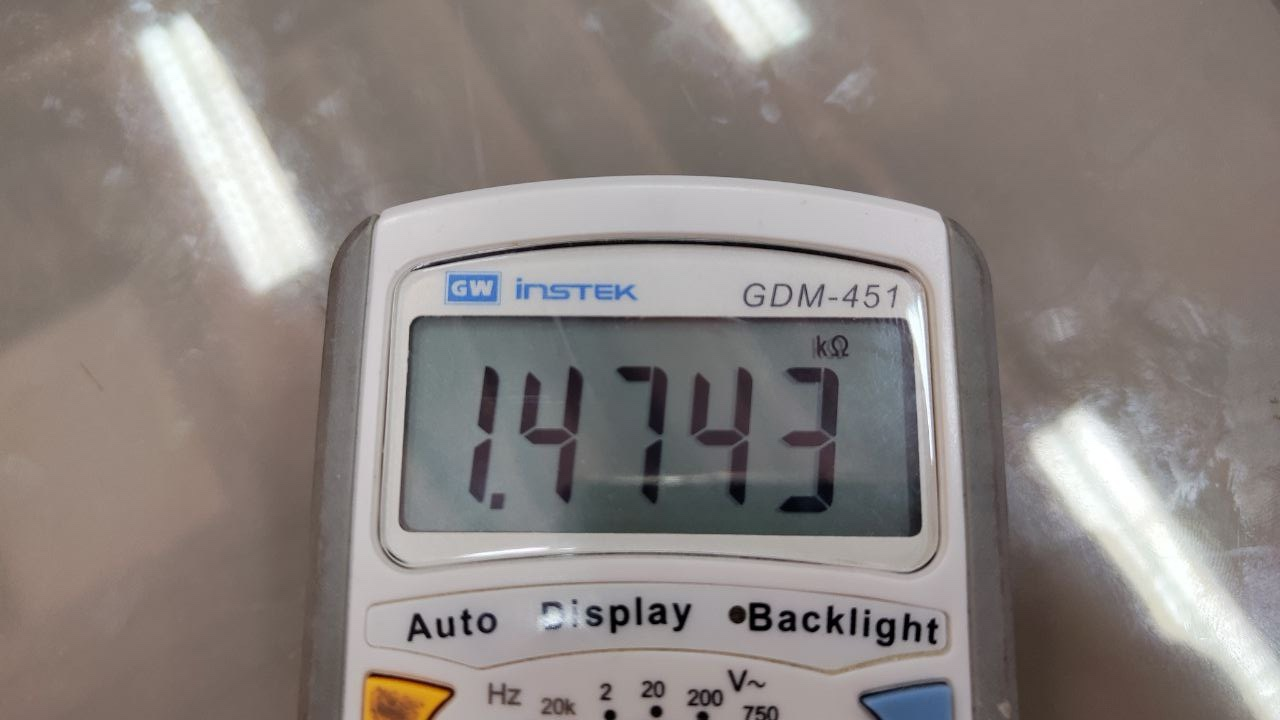
\includegraphics[scale=\PicScale,angle=0]{Fig/21.jpeg}
                \caption{The exact value of $R$.}
            \end{figure}
            \begin{figure}[H]
                \centering
                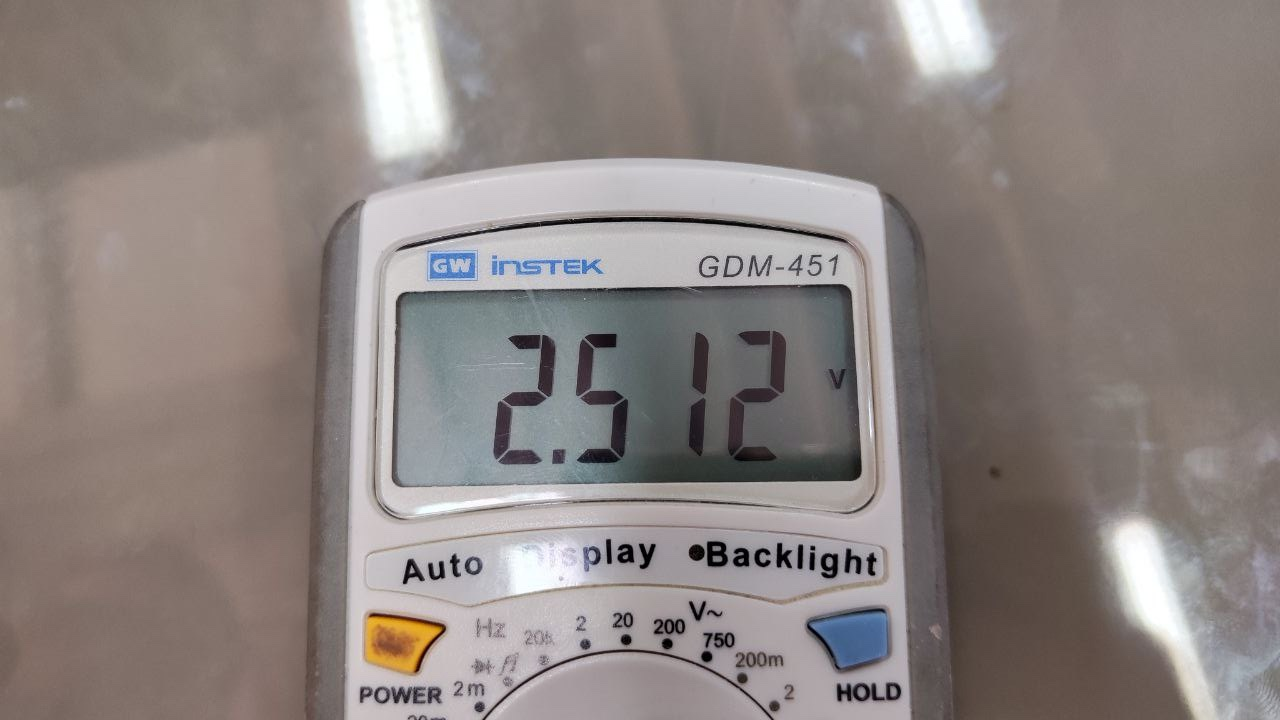
\includegraphics[scale=\PicScale,angle=0]{Fig/22.jpeg}
                \caption{The exact value of $v$ of $R$.}
            \end{figure}
        }
    \end{subquestion}

    %--------------------------------------------
    \begin{subquestion}{Connect a $1$ k$\Omega$ and a $2.2$ k$\Omega$ resistor to the port and measure the corresponding consumed powers. Discuss the results and verify the maximum power transfer theorem.}
        \answer{
            \begin{figure}[H]
                \centering
                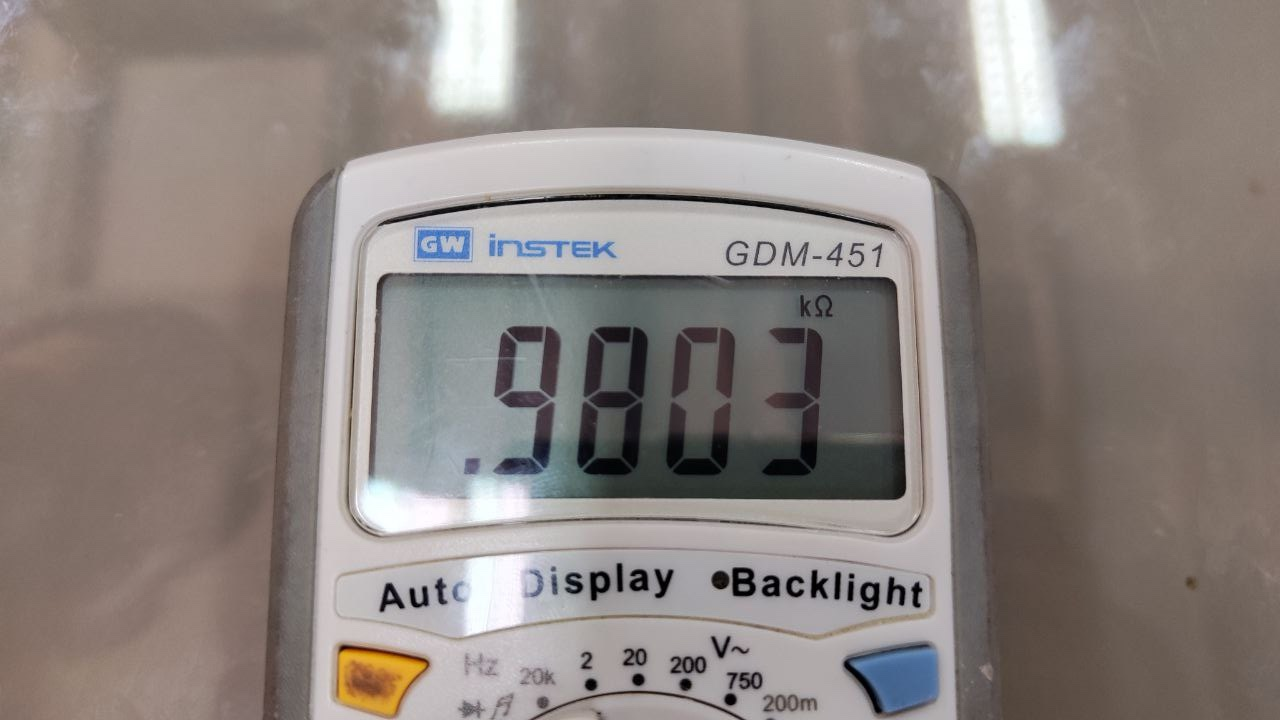
\includegraphics[scale=\PicScale,angle=0]{Fig/23.jpeg}
                \caption{The exact value of $R$.}
            \end{figure}
            \begin{figure}[H]
                \centering
                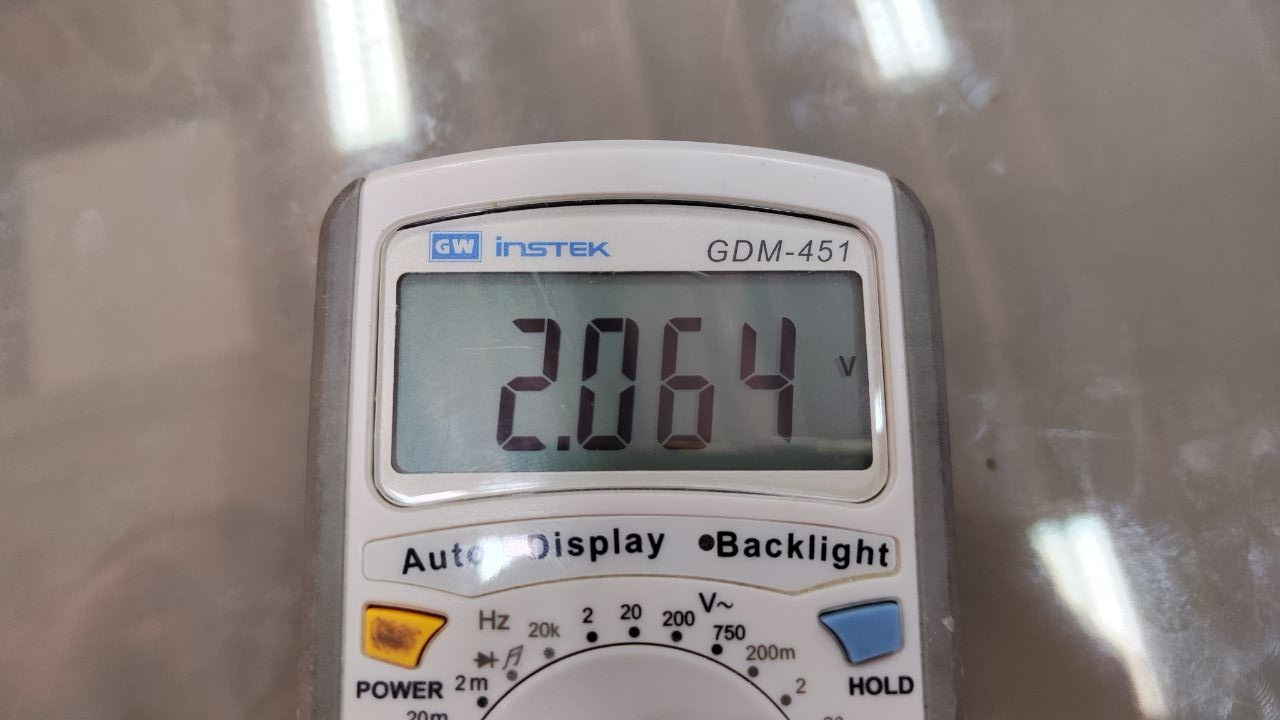
\includegraphics[scale=\PicScale,angle=0]{Fig/24.jpeg}
                \caption{The exact value of $v$ of $R$.}
            \end{figure}
            \begin{figure}[H]
                \centering
                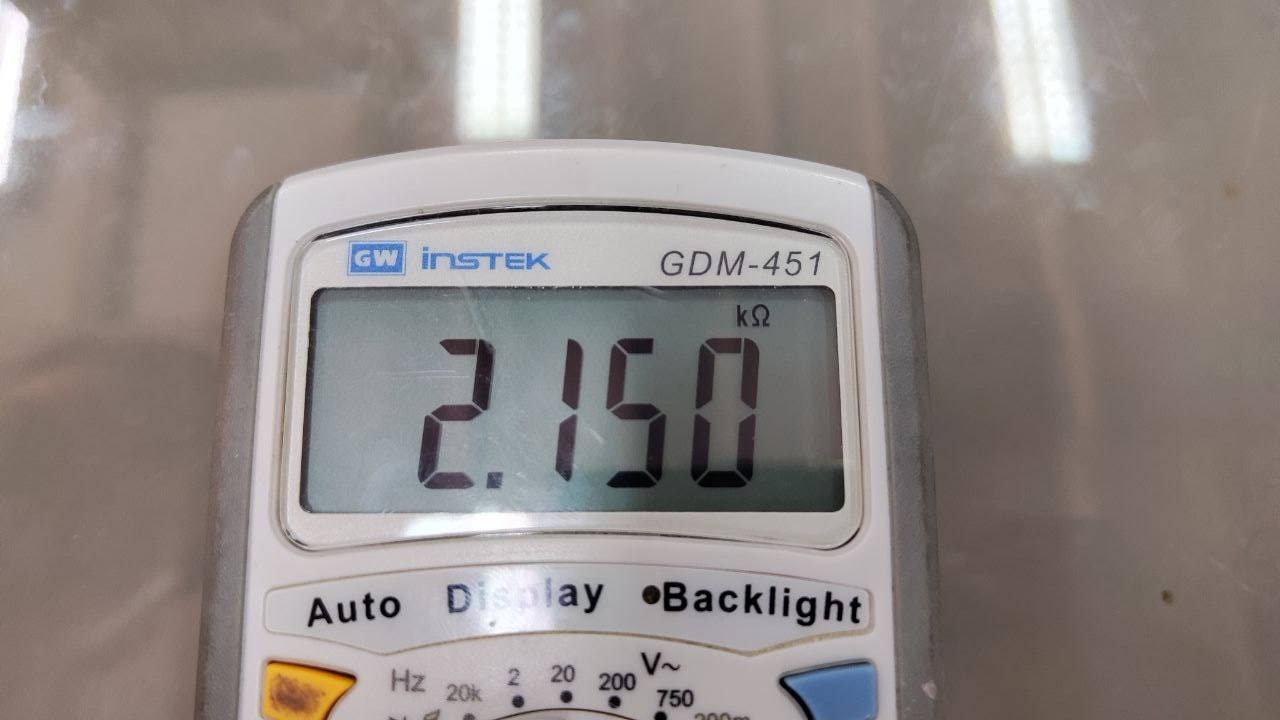
\includegraphics[scale=\PicScale,angle=0]{Fig/25.jpeg}
                \caption{The exact value of $R$.}
            \end{figure}
            \begin{figure}[H]
                \centering
                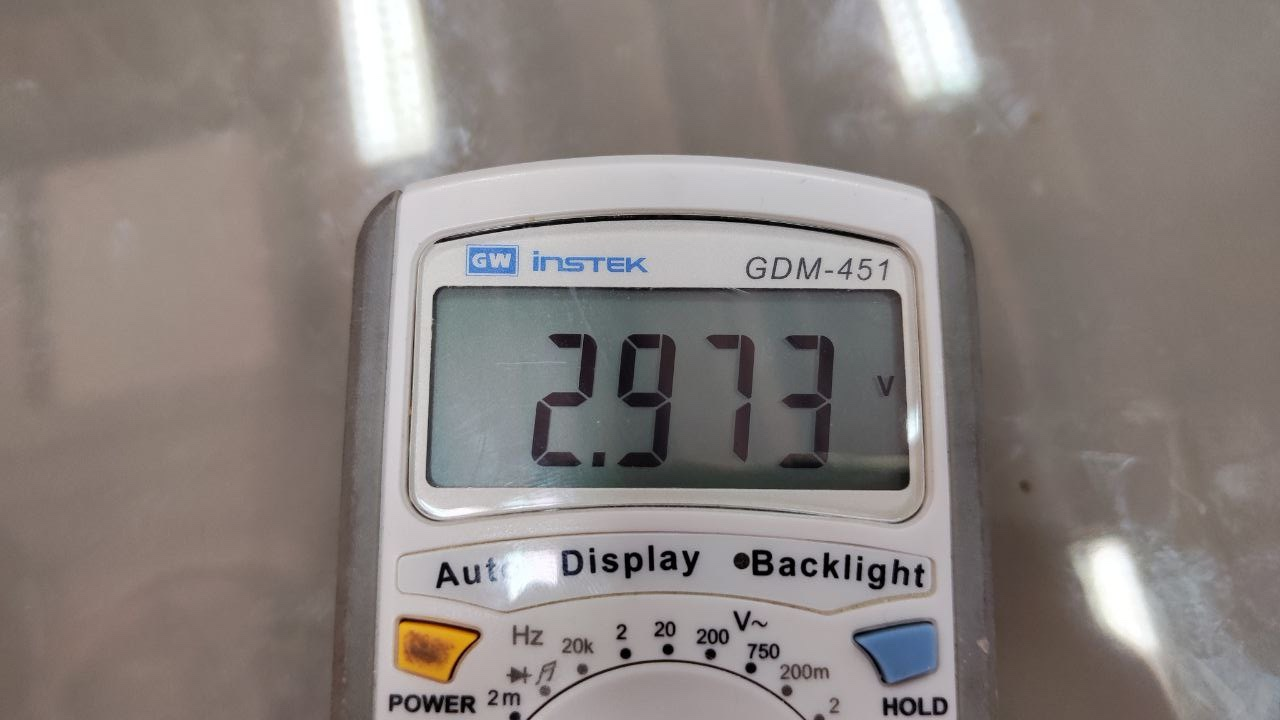
\includegraphics[scale=\PicScale,angle=0]{Fig/26.jpeg}
                \caption{The exact value of $v$ of $R$.}
            \end{figure}
        }
    \end{subquestion}


\end{question}

\assignmentSection{Bonus Experiments}

%----------------------------------------------------------------------------------------
%	QUESTION 4
%----------------------------------------------------------------------------------------
\begin{question}

    \questiontext{A Zener diode is a special type of diode designed to reliably allow current to flow backwards when a certain set reverse voltage, known as the Zener voltage, is reached. The characteristic curve of a typical Zener diode is shown in Fig. \ref{fig:zener}. Explain how a Zener diode can be used as a voltage source. Is there any practical or analytical limitation on a voltage source created by a Zener diode?}

    \begin{figure}[H]
        \centering
        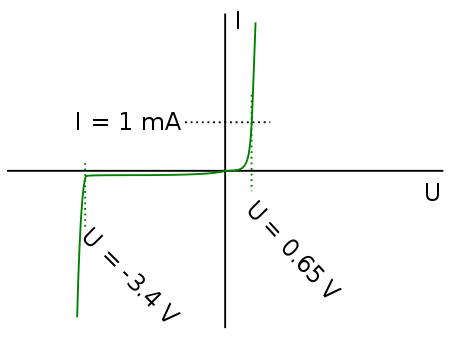
\includegraphics[scale=0.5,angle=0]{Fig/zener.png}
        \caption{Typical characteristic of a Zener diode.} \label{fig:zener}
    \end{figure}

    \answer{}

\end{question}
%----------------------------------------------------------------------------------------
%	QUESTION 5
%----------------------------------------------------------------------------------------

\begin{question}

    \questiontext{Consider the typical characteristic curve of a Zener diode.}
    %---------------------------------------------------------------------------------------
    \begin{subquestion}{Propose a piecewise linear approximation for the characteristic curve using vertical and/or horizontal lines. The forward and (Zener) breakdown voltages should be included in the approximation. }

        \answer{}

    \end{subquestion}

    %----------------------------------------------------------------------------------------
    \begin{subquestion}{Use the proposed piecewise linear approximation to suggest a model for the Zener diode. You may use ideal diodes, independent sources, or passive LTI resistors in your model. }

        \answer{}

    \end{subquestion}

    %----------------------------------------------------------------------------------------
    \begin{subquestion}{Use PSpice simulation to verify the accuracy of the suggested model for D02CZ10 zener diode with the forward and breakdown voltages around $0.7$ and $-10$ V. }

        \answer{}

    \end{subquestion}

\end{question}



%----------------------------------------------------------------------------------------
%	QUESTION 6
%----------------------------------------------------------------------------------------

\begin{question}

    \questiontext{Return your work report by filling the \LaTeX template of the manual. Include useful and high-quality images to make the report more readable and understandable.}

\end{question}

%----------------------------------------------------------------------------------------

\end{document}
